% Created 2021-04-10 sáb 14:30
% Intended LaTeX compiler: pdflatex
\documentclass{SelfArx}
  \usepackage[T1]{fontenc}
\usepackage[utf8]{inputenc}
\usepackage{booktabs}
\renewcommand{\arraystretch}{1.1} % Unclear
\usepackage{graphicx}
\usepackage{float}
\usepackage{amsmath}
\usepackage{csquotes}
\setlength{\fboxrule}{0.75pt} % Width of the border around the abstract
\usepackage{longtable}
\definecolor{color1}{RGB}{0,0,90} % Color of the article title and sections
\definecolor{color2}{RGB}{0,20,20} % Color of the boxes behind the abstract and headings
\usepackage[portuguese, english]{babel} % Specify a different language here - english by default
\usepackage{lipsum} % Required to insert dummy text. To be removed otherwise
\usepackage[backend=biber,%
style = abnt,%
noslsn, %
isbn = false,
url = false,
extrayear, %
uniquename=init,%
giveninits, %
justify, %
sccite,%
scbib, %
sorting=nyt,
% mergedate=compact,
% natbib=true,
repeattitles, %
maxcitenames=3]{biblatex}
\AtEveryBibitem{%
\clearfield{urlyear}
\clearfield{urlmonth}
\clearfield{note}
\clearfield{issn} % Remove issn
\clearfield{doi} % Remove doi
\ifentrytype{online}{}{% Remove url except for @online
\clearfield{url}
}
}
\usepackage{multirow, numprint}
\date{}
\title{Dados: O PIB da pandemia e cenários para 2021}
\begin{document}

\JournalInfo{Nota de Conjuntura No 17} % Journal information
\Archive{} % Additional notes (e.g. copyright, DOI, review/research article)

\Authors{Pedro Paulo Zahluth Bastos\textsuperscript{1}*, Gabriel Petrini\textsuperscript{2}, Lorena Dourado\textsuperscript{3}} % Authors
\affiliation{\textsuperscript{1}\textit{Professor do Instituto de Economia Unicamp}} % Author affiliation
\affiliation{\textsuperscript{2}\textit{Doutorando do Instituto de Economia  Unicamp}} % Author affiliation
\affiliation{\textsuperscript{3}\textit{Graduanda do Instituto de Economia Unicamp}} % Author affiliation
\affiliation{*\textbf{E-mail}: ppzbastos@gmail.com} % Corresponding author

\newcommand{\keywordname}{Palavras-chave} % Defines the keywords heading name

\Abstract{
\begin{itemize}
\item O PIB do Brasil em 2020 reforça o consenso científico que beira a unanimidade: é a pandemia que deprime a economia, e não as iniciativas de saúde pública capazes de controlá-la. A contração da economia e da mobilidade voluntária precederam ações de distanciamento social estritas, que chegaram atrasadas para controlar os vários picos da pandemia e, assim, criar condições para recuperação econômica sustentada.
\item A bibliografia internacional sobre o impacto econômico da pandemia indica que ações de distanciamento social moderadas têm grande impacto econômico negativo que reforça o efeito do distanciamento voluntário, mas não são eficientes para reduzir a taxa de crescimento das infecções. Já ações de distanciamento social estritas conseguem sim reduzir as infecções, mas tem impacto econômico negativo pequeno na margem, pois a maior parte do impacto já tinha sido produzido pelo distanciamento voluntário e pela ação de distanciamento social moderada.
\item A conclusão é óbvia: ao invés de ficar parado torcendo para que a economia não despenque – pois ela vai despencar mesmo sem lockdowns rigorosos -, é melhor decretar lockdowns rigorosos o mais cedo possível, acompanhando-o de ações para evitar novos surtos (testagem, rastreio de contatos e isolamento seletivo). Assim, a redução brusca das infecções pode criar condições epidemiológicas para uma recuperação econômica sustentada, pois enquanto houver
risco de infecção haverá distanciamento voluntário. A médio prazo, portanto, não há conflito entre atividade econômica e controle da pandemia.
\item A economia brasileira confirma o padrão internacional. Estimamos o distanciamento social voluntário avaliando dados de mobilidade nos estados brasileiros e comparando-os com alterações nas ações de distanciamento social. Em muitos estados há sincronia quase perfeita entre as curvas de mobilidade e de número de casos independentemente de mudanças significativas na ação de distanciamento social, o que se explica pelo distanciamento voluntário.
\item Em razão do distanciamento voluntário, a recuperação econômica iniciada no terceiro trimestre desacelerou no quarto antes mesmo da interrupção do auxílio emergencial. A pandemia, tornando-se endemia, limitou a retomada da demanda e do emprego em serviços no último trimestre em razão dos riscos de transmissão, a despeito do relaxamento das ações de distanciamento social. Logo, tanto o distanciamento social quanto as políticas de defesa da renda foram mitigadas ou suspendidas cedo demais, e não foram acompanhadas nem sucedidas por ações para evitar novos surtos (testagem, rastreio de contatos e isolamento seletivo) por falta de coordenação nacional.
\item Como esperado, o recrudescimento da pandemia em 2021 foi novamente acompanhado da piora dos dados de mobilidade e dos indicadores econômicos. O indicador da OCDE para a semana concluída em 03 de abril de 2021 aponta para uma contração de 7,5\%, uma deterioração de 6 p.p. em menos de dois meses que leva o índice ao patamar do final de julho de 2020, quando ocorria o primeiro pico da pandemia em São Paulo e no Rio de Janeiro.
\item A gravidade da conjuntura aumenta a urgência da combinação de políticas de saúde pública com nova rodada de estímulos fiscais. Tal rodada deveria ser muito superior à retomada do auxílio emergencial em 06 de abril, que estimamos representar um choque negativo de 3\% do PIB em relação aos valores de 2020.
\item Sem controle da pandemia, a economia brasileira deve participar timidamente, na melhor das hipóteses, da recuperação do PIB dos grandes parceiros comerciais que ampliam a vacinação e controlam a pandemia em 2021. A pior das hipóteses, contudo, é cada vez mais provável.
\end{itemize}
}
\renewcommand{\abstractname}{Sumário Executivo} % Defines the keywords heading name
\flushbottom % Makes all text pages the same height
\maketitle % Print the title and abstract box
\thispagestyle{empty} % Removes page numbering from the first page
\onecolumn
\bibliography{refs}

\section*{Indicadores de antecedente}
\label{sec:org4e39b7b}
\subsection*{IBC-Br (acumulado 12 meses vs 12 meses anteriores)}
\label{sec:org28f78fb}

\begin{center}
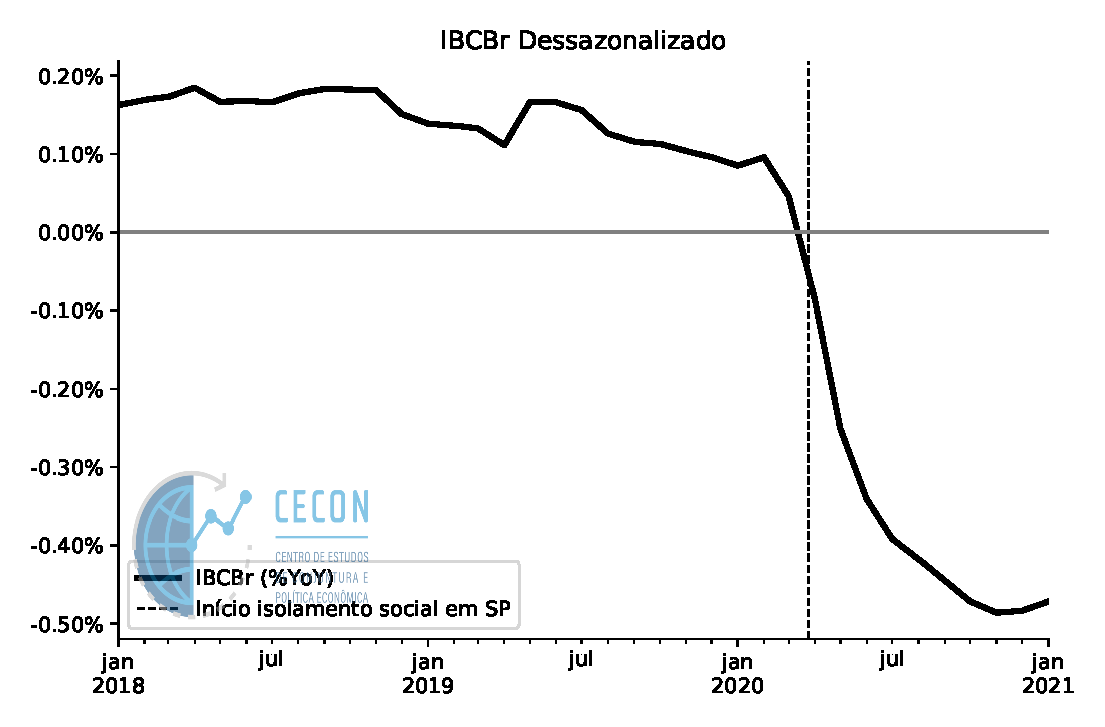
\includegraphics[width=.9\linewidth]{./figs/Antecedente/IBCBr.pdf}
\end{center}

\subsection*{Tráfego de veículos pesados nas estradas pedagiadas - ABCR - Dados dessazonalizados}
\label{sec:org6356d69}


\begin{center}
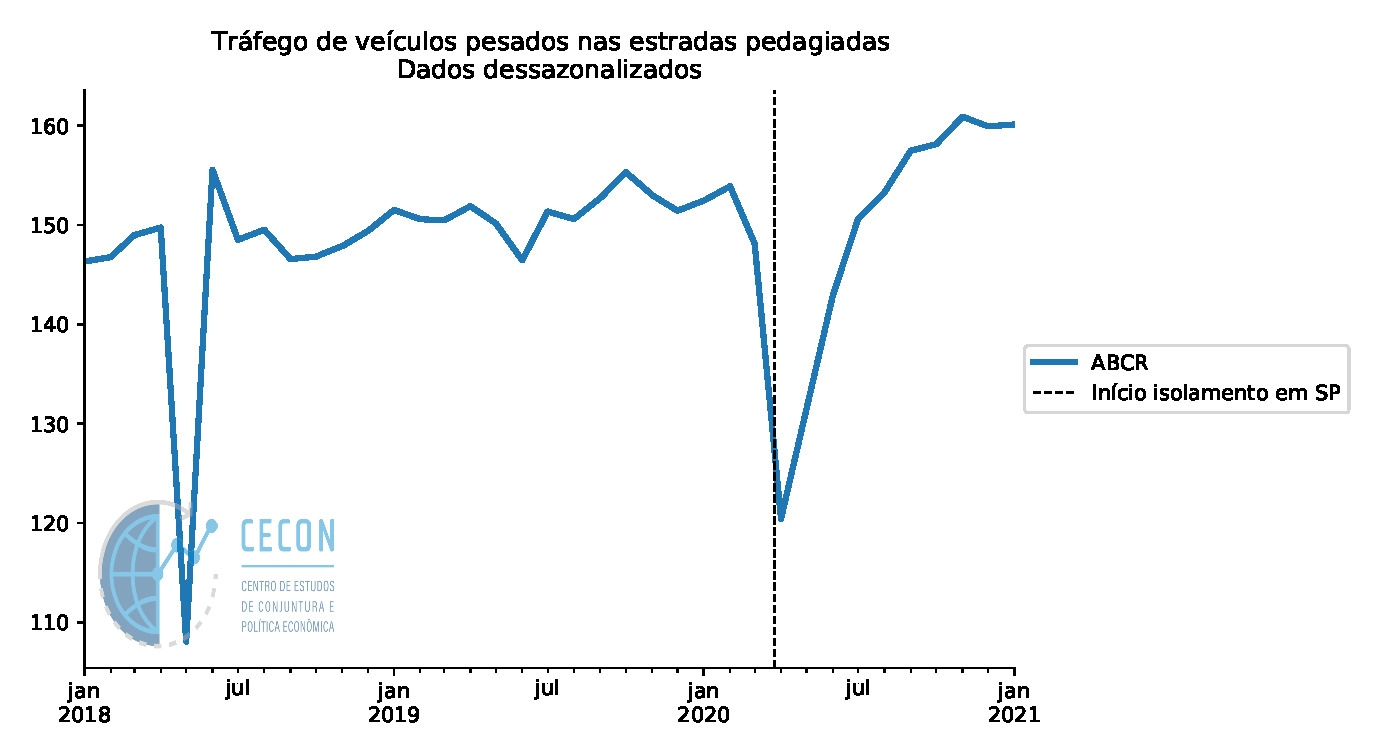
\includegraphics[width=.9\linewidth]{./figs/Setoriais/TrafegoPedagio.pdf}
\end{center}


\section*{Dados de alta frequência}
\label{sec:orga343f68}

\subsection*{Bloomberg adaptado ao COVID-19 (\href{https://www.bloomberg.com/news/articles/2020-11-13/alternative-data-show-activity-crashes-as-virus-resurges-chart}{Link})}
\label{sec:org9d14cbc}

\subsection*{Google Reports: Brasil}
\label{sec:orgfe161d7}

\subsubsection*{Brasil}
\label{sec:org19da8f8}

\begin{center}
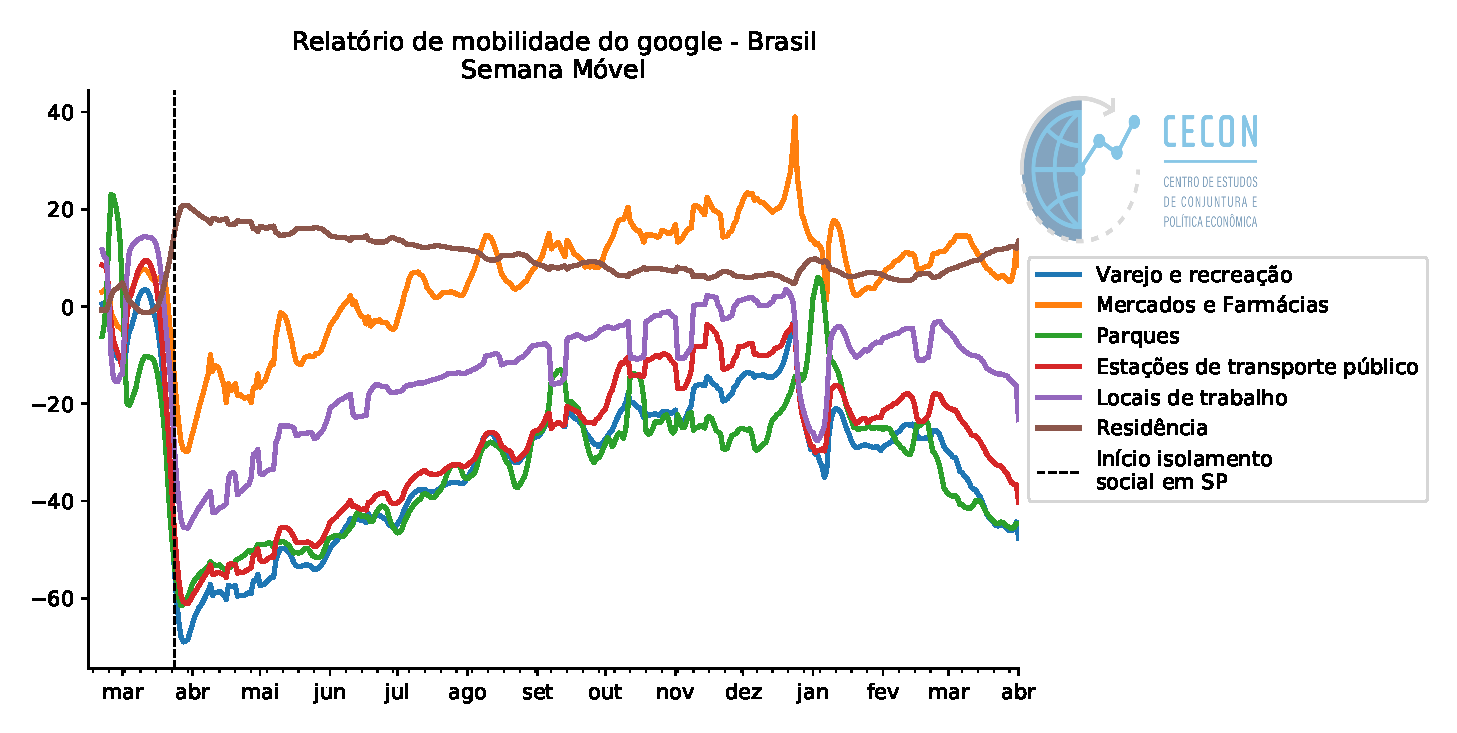
\includegraphics[width=.9\linewidth]{./figs/Granulares/GoogleReport_Brasil.pdf}
\end{center}

\subsubsection*{Estado de São Paulo}
\label{sec:org9abd089}

\begin{center}
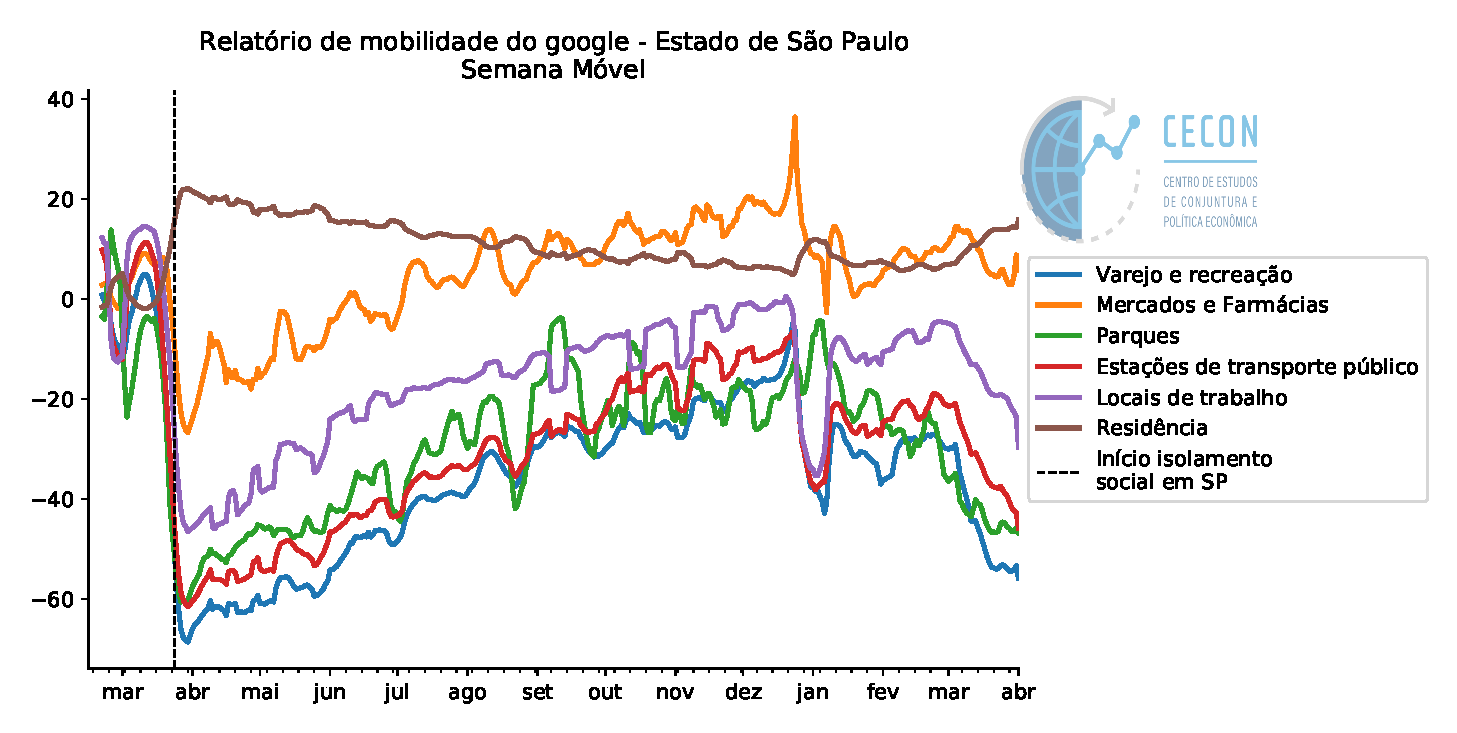
\includegraphics[width=.9\linewidth]{./figs/Granulares/GoogleReport_EstadoSP.pdf}
\end{center}

\subsubsection*{Cidade de São Paulo}
\label{sec:orgdc33422}

\begin{center}
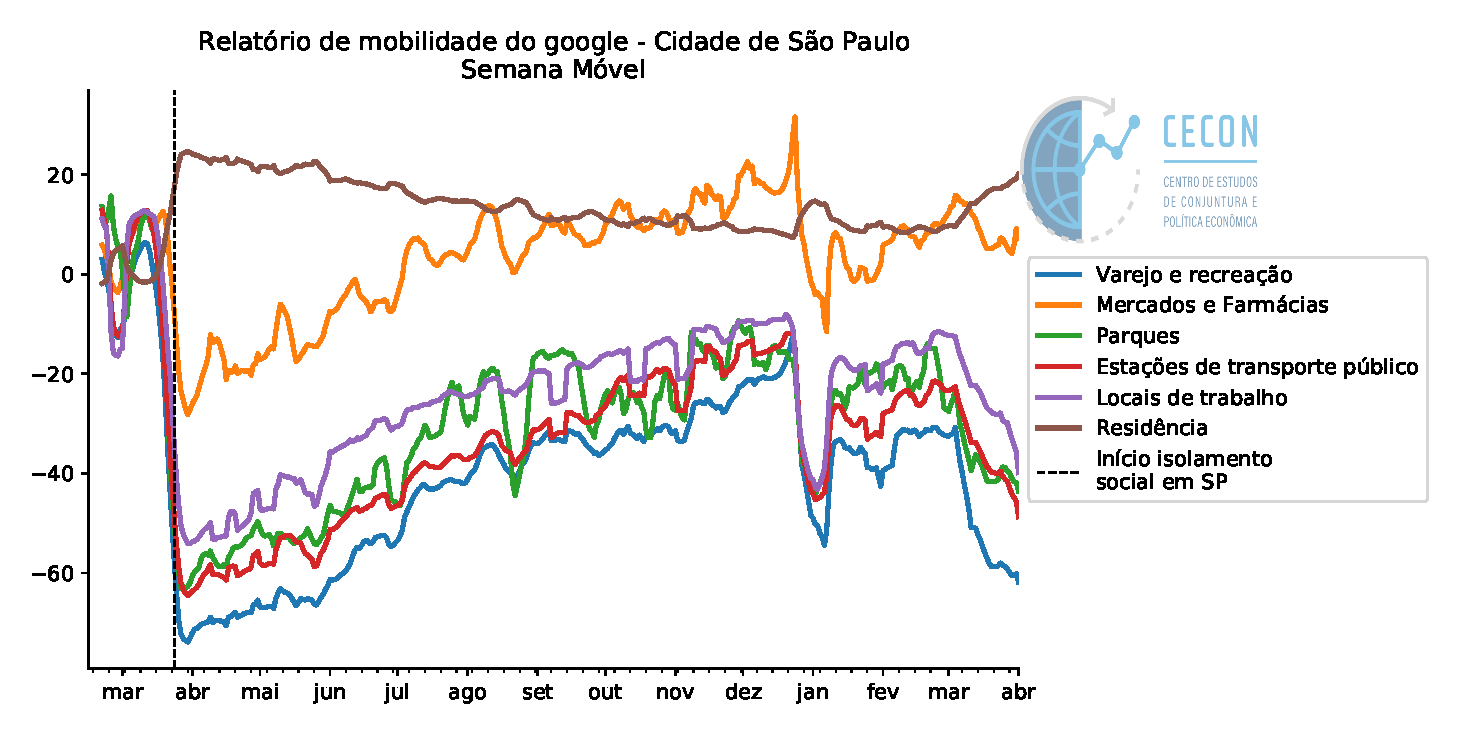
\includegraphics[width=.9\linewidth]{./figs/Granulares/GoogleReport_CidadeSP.pdf}
\end{center}

\subsection*{Apple: Tendências de mobilidade}
\label{sec:org20b458f}

\begin{center}
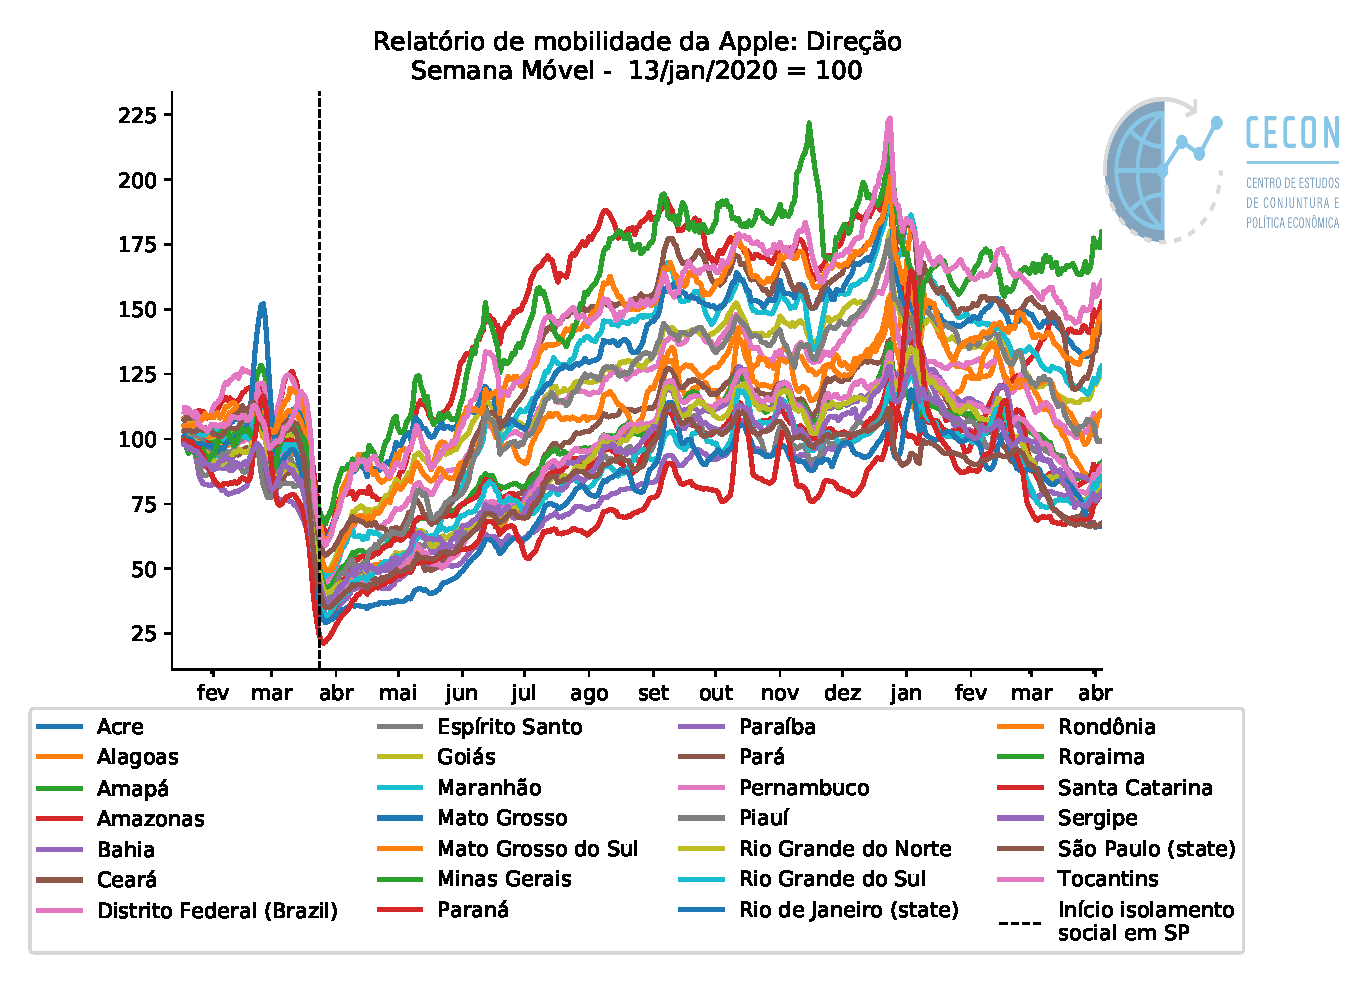
\includegraphics[width=.9\linewidth]{./figs/Granulares/AppleReport_Brasil.pdf}
\end{center}

\subsection*{Waze: \(\Delta \%\) Km}
\label{sec:org3c49aa6}

\begin{center}
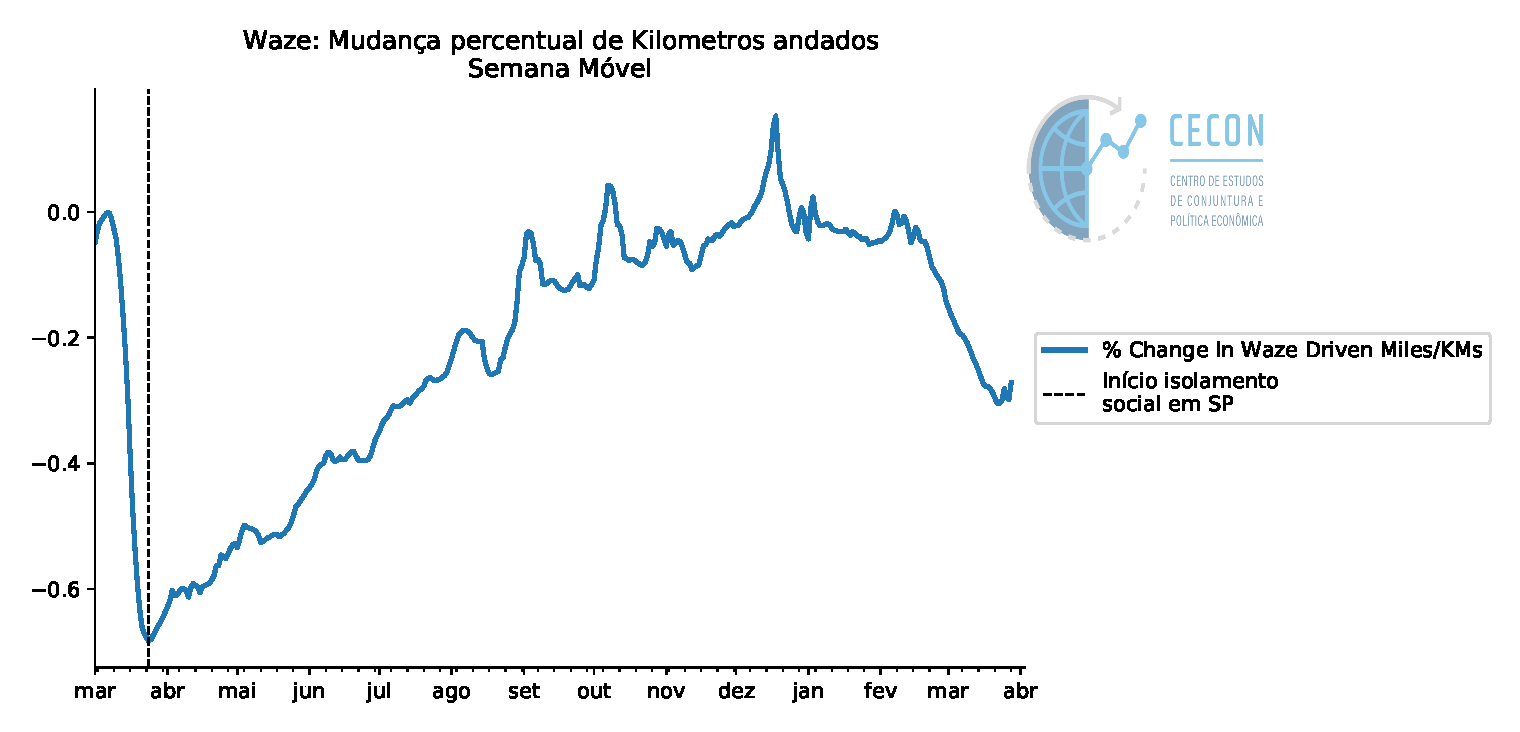
\includegraphics[width=.9\linewidth]{./figs/Granulares/Waze_Brasil.pdf}
\end{center}

\subsection*{TomTom: Congestionamento}
\label{sec:org802702b}

\begin{center}
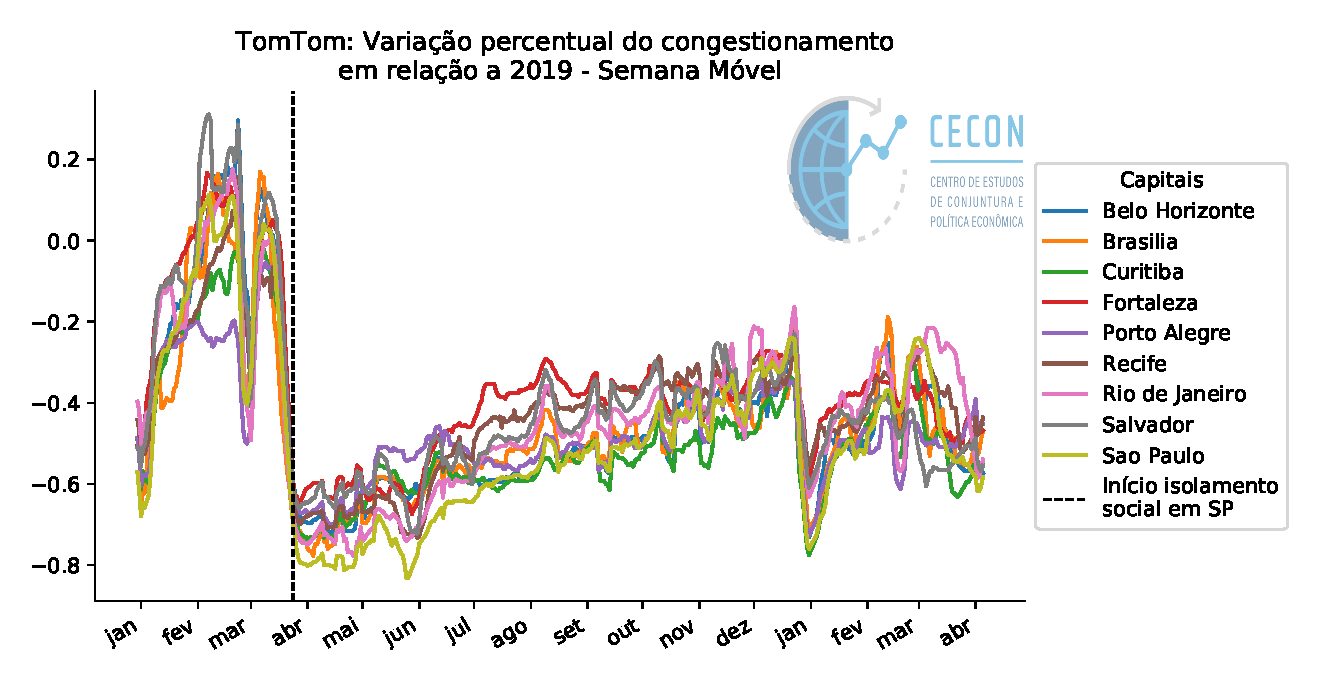
\includegraphics[width=.9\linewidth]{./figs/Granulares/TomTom_Brasil.pdf}
\end{center}

\section*{Atividade}
\label{sec:orgefb06dc}



\subsection*{Trimestre Contra trimestre imediatamente anterior}
\label{sec:org664c8b1}

\begin{center}
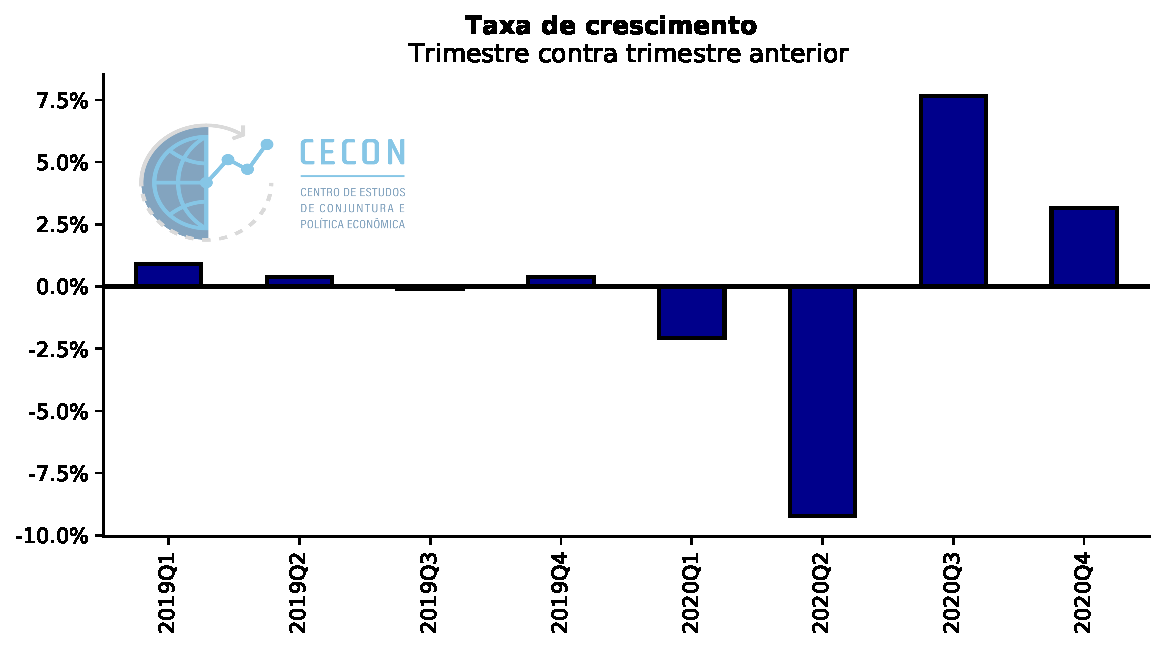
\includegraphics[width=.9\linewidth]{./figs/PIB/PIB.pdf}
\end{center}

\subsection*{Trimestre Contra mesmo trimestre do ano anterior}
\label{sec:org704e767}

\begin{center}
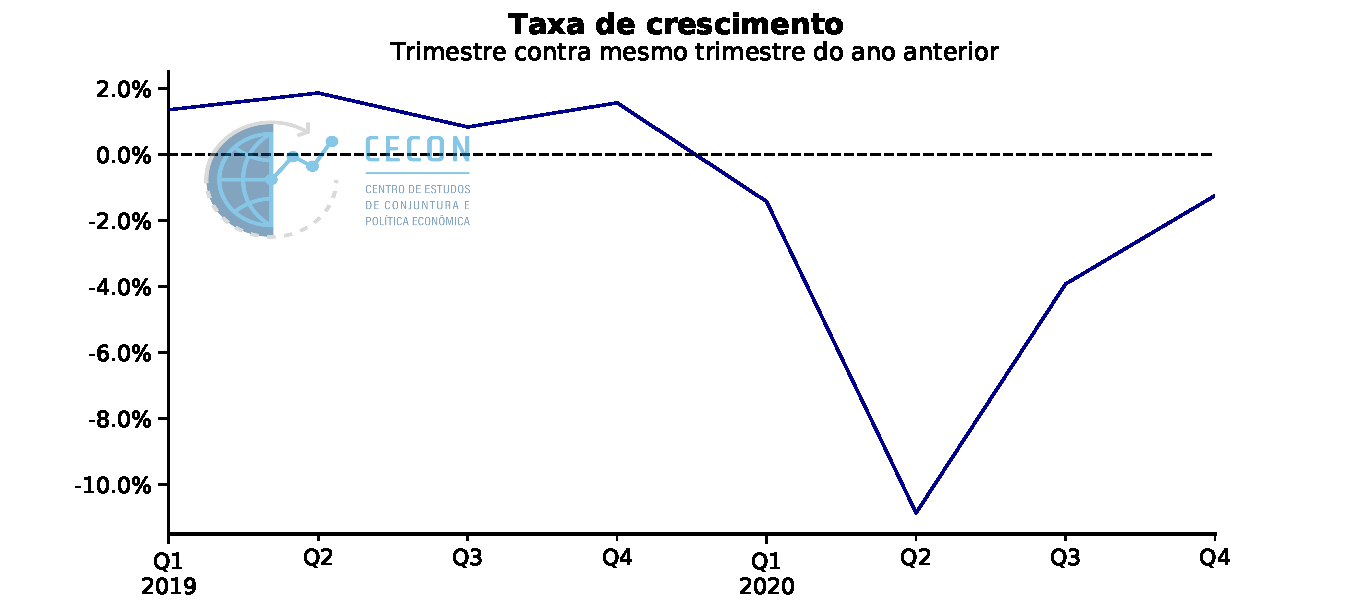
\includegraphics[width=.9\linewidth]{./figs/PIB/PIB_YoY.pdf}
\end{center}

\subsection*{Agropecuária}
\label{sec:orgc914f7f}

\begin{center}
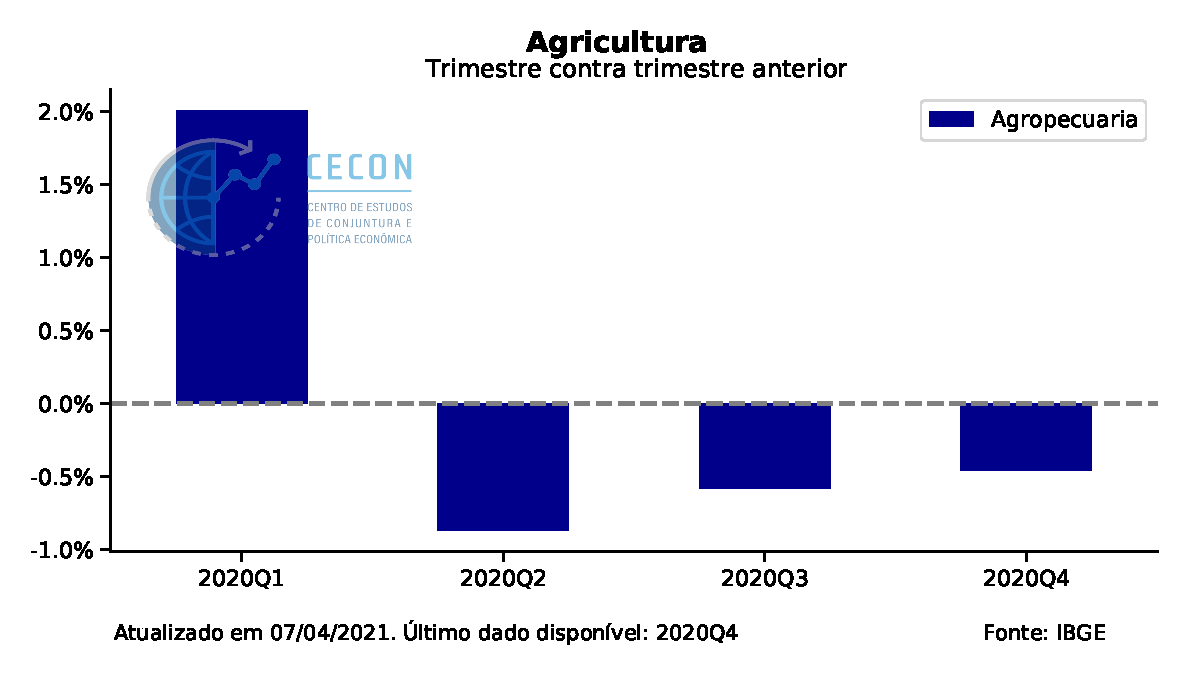
\includegraphics[width=.9\linewidth]{./figs/PIB/Agropecuaria.pdf}
\end{center}

\subsection*{Indústria}
\label{sec:org87c9e11}

\begin{center}
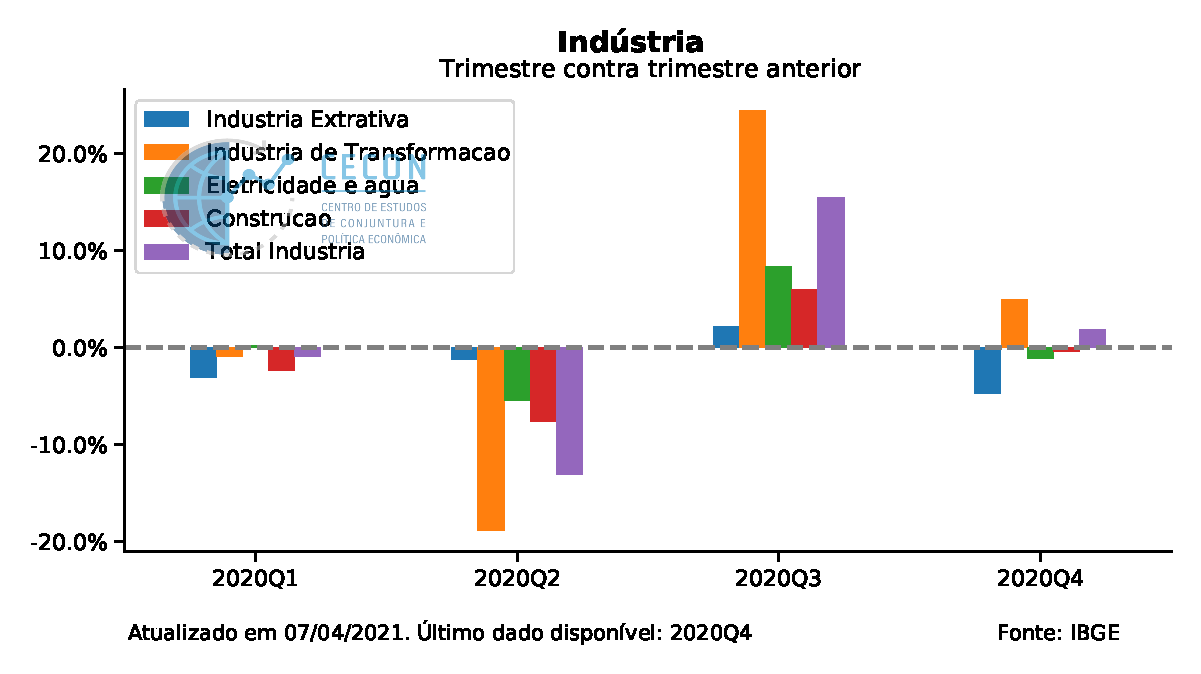
\includegraphics[width=.9\linewidth]{./figs/PIB/Industria.pdf}
\end{center}


\subsection*{Serviços}
\label{sec:org2fd4ec2}

\begin{center}
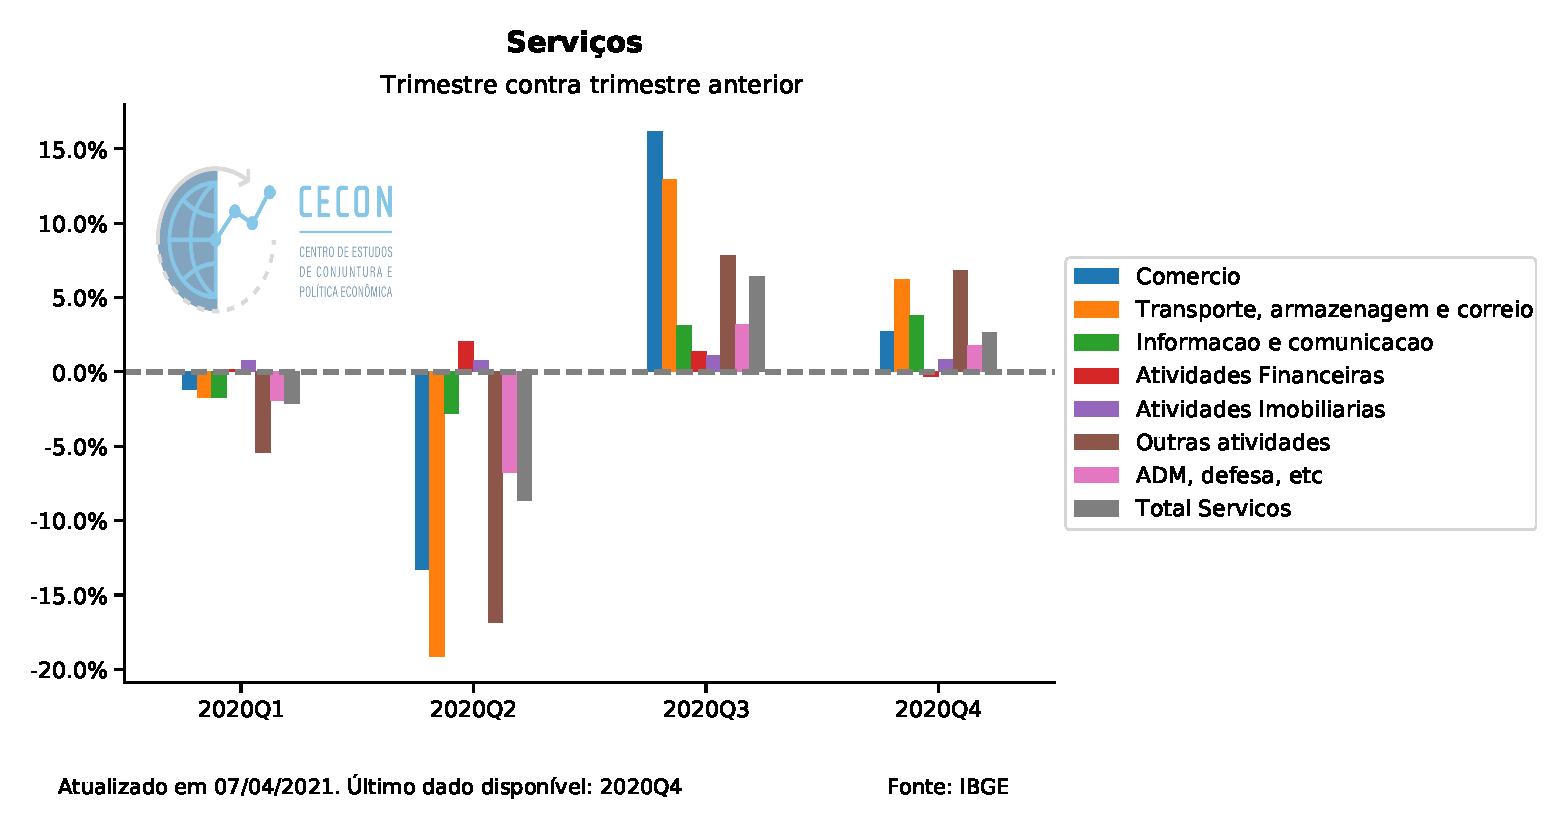
\includegraphics[width=.9\linewidth]{./figs/PIB/Servicos.pdf}
\end{center}

\subsection*{Demanda}
\label{sec:orgdc97a2c}

\begin{center}
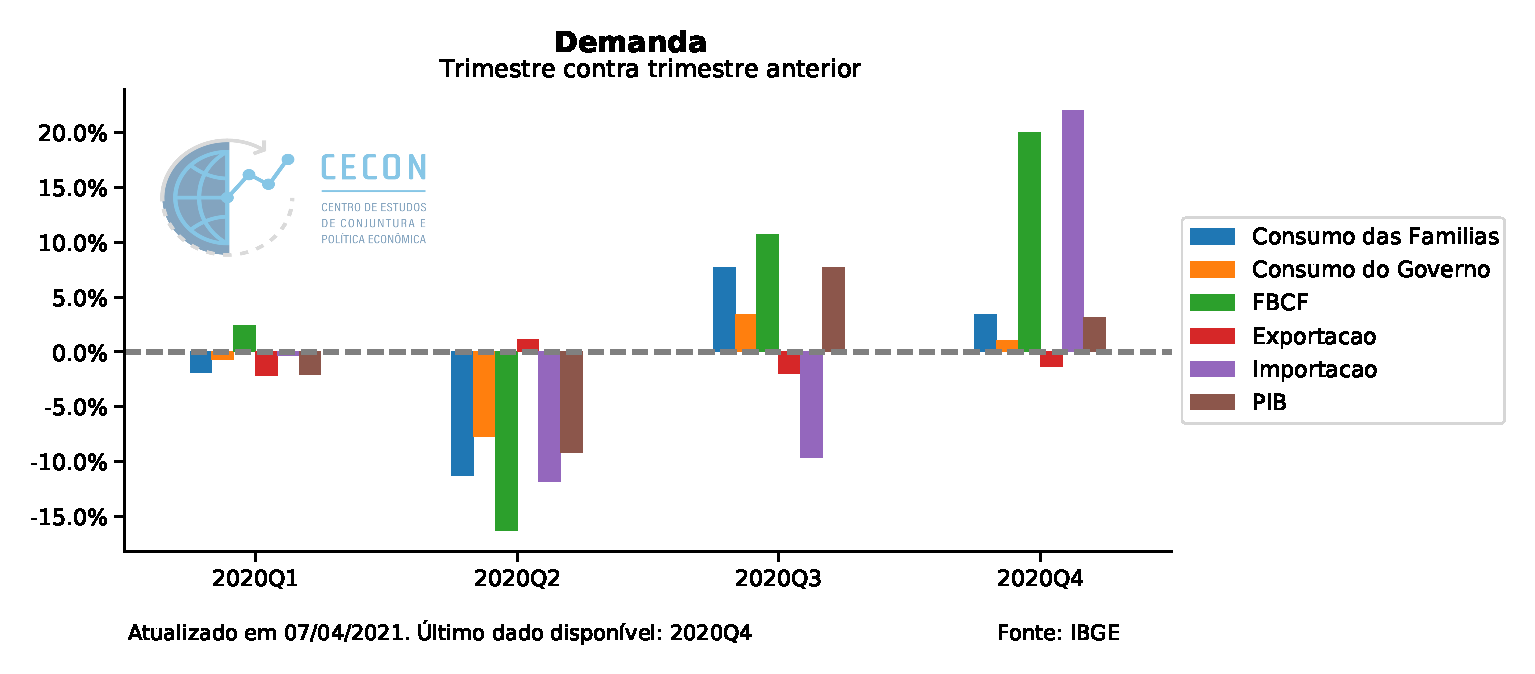
\includegraphics[width=.9\linewidth]{./figs/PIB/Demanda.pdf}
\end{center}

\subsection*{Oferta}
\label{sec:org571b86b}


\begin{center}
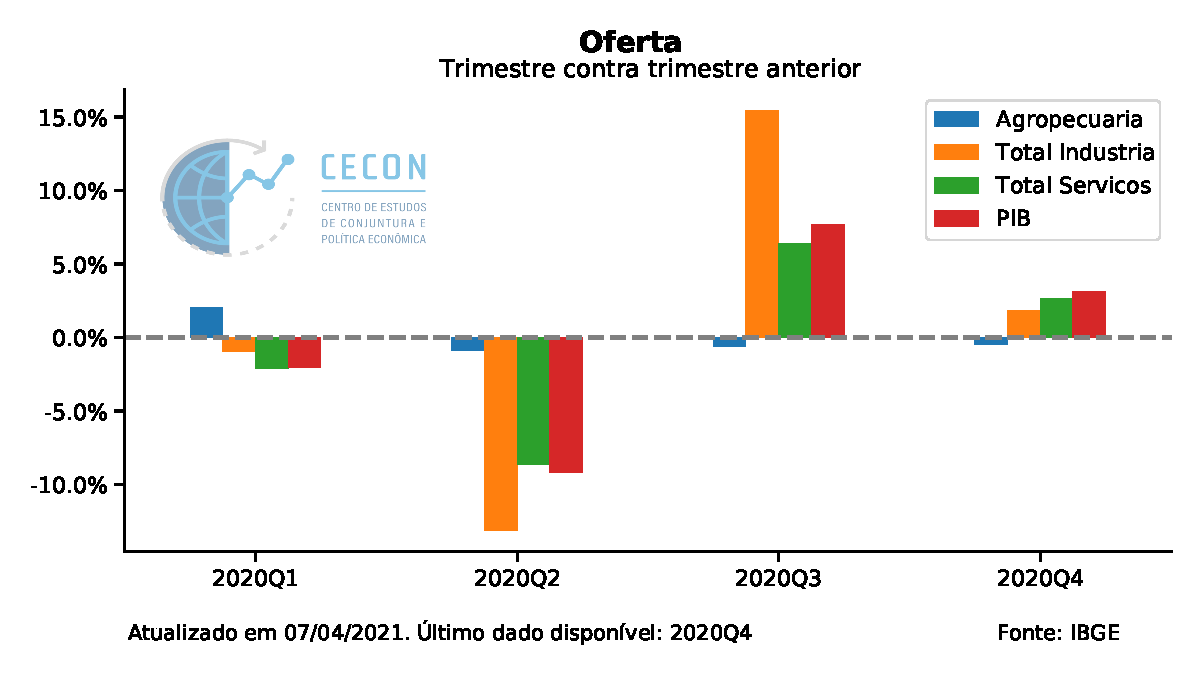
\includegraphics[width=.9\linewidth]{./figs/PIB/Oferta.pdf}
\end{center}


\subsection*{Contribuição para variação: Demanda}
\label{sec:org588a030}

\begin{center}
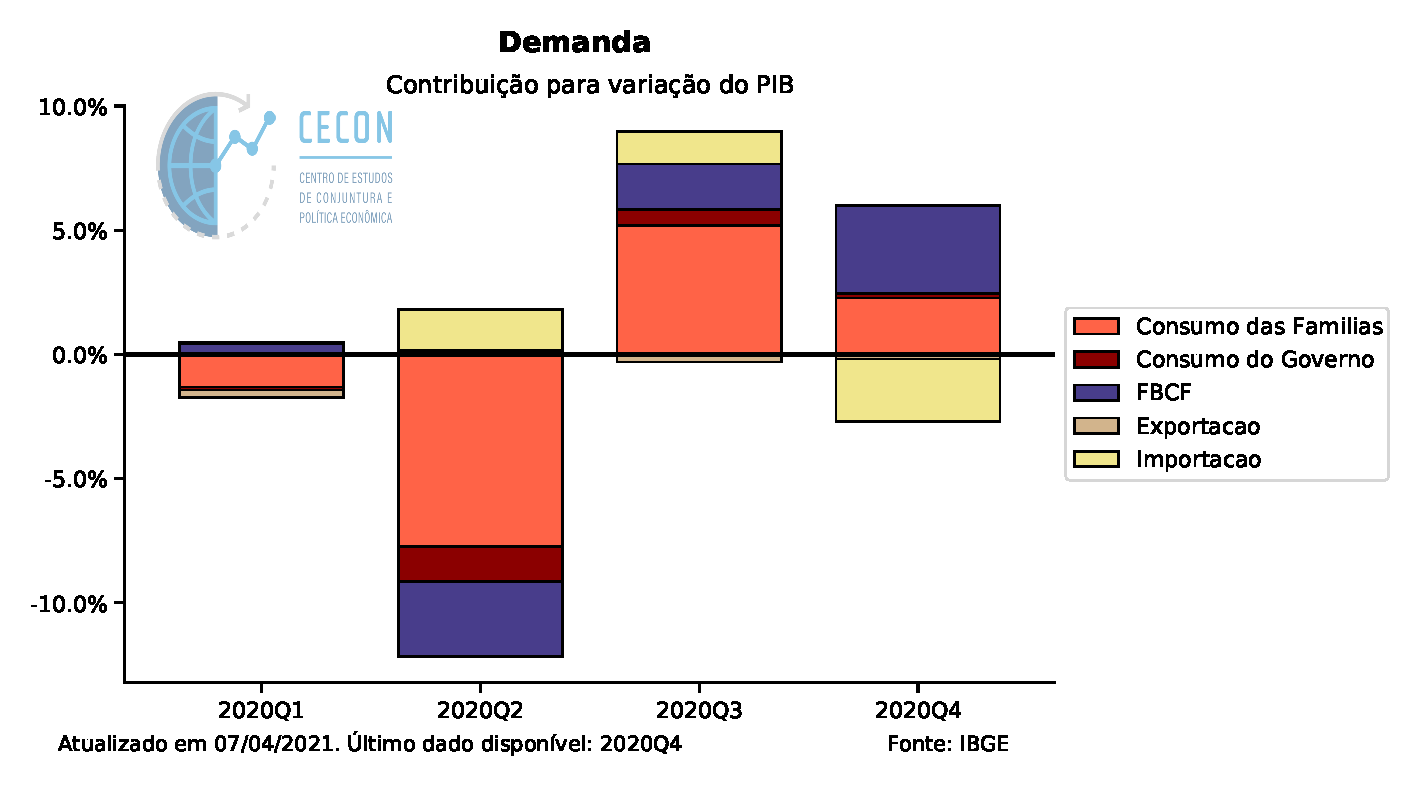
\includegraphics[width=.9\linewidth]{./figs/PIB/Contrib_Demanda.pdf}
\end{center}

\subsection*{Contribuição para variação: Oferta}
\label{sec:org802858d}

\begin{center}
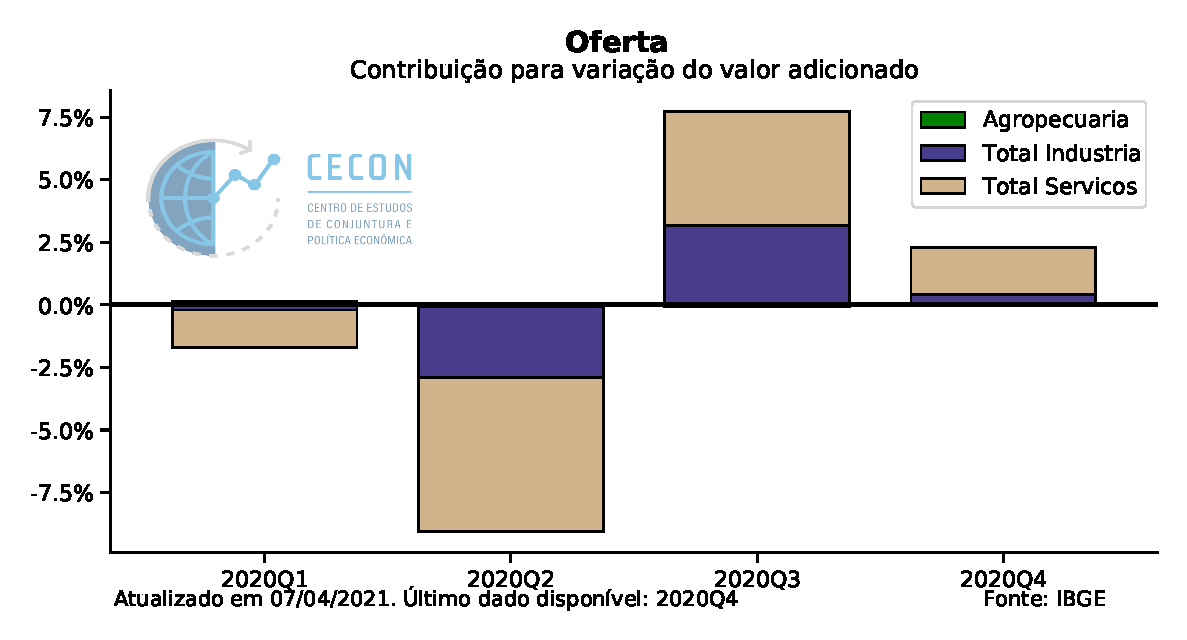
\includegraphics[width=.9\linewidth]{./figs/PIB/Contrib_Oferta.pdf}
\end{center}


\subsection*{Contribuição para variação: Serviços}
\label{sec:org5f08c3f}

\begin{center}
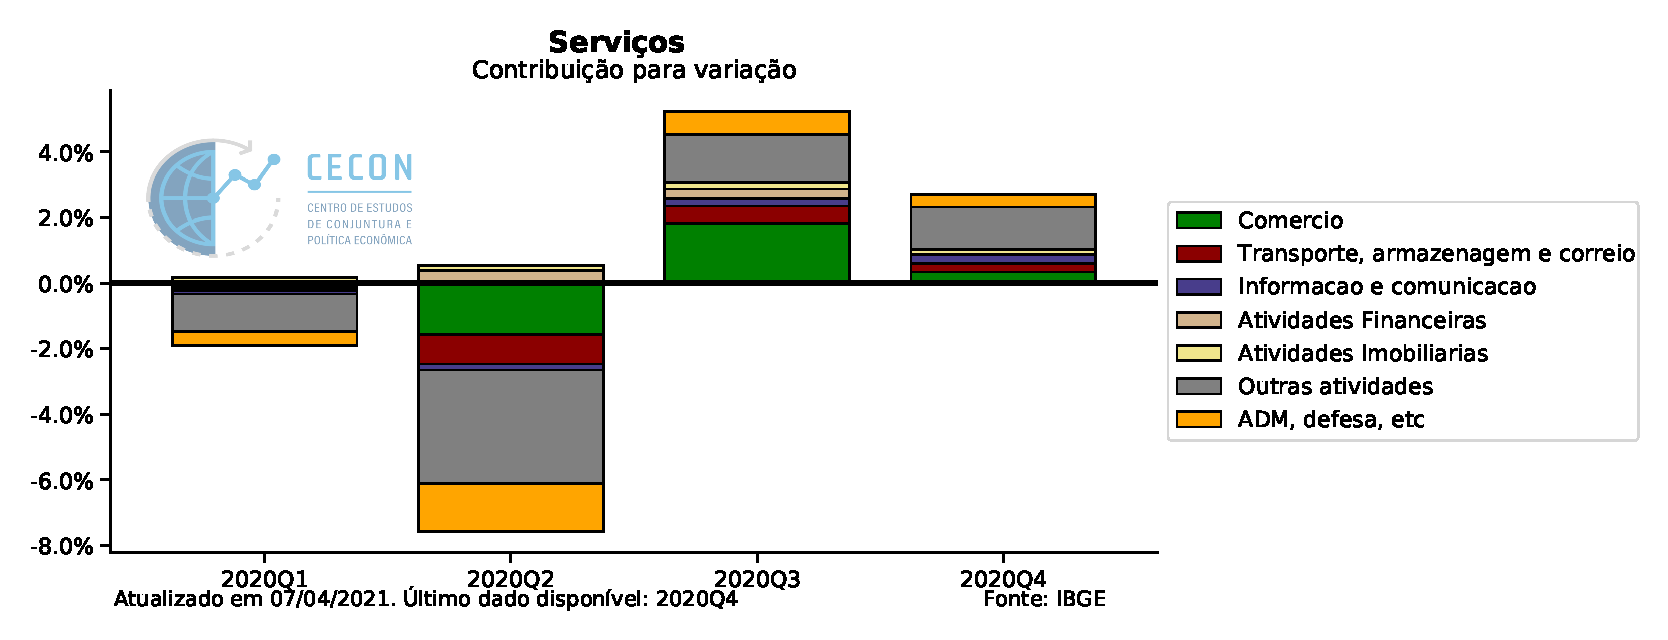
\includegraphics[width=.9\linewidth]{./figs/PIB/Contrib_Servicos.pdf}
\end{center}

\subsection*{Acumulado no ano (sem ajuste)}
\label{sec:orgf3d5f06}

\subsubsection*{Serviços}
\label{sec:org0d8997d}

\begin{center}
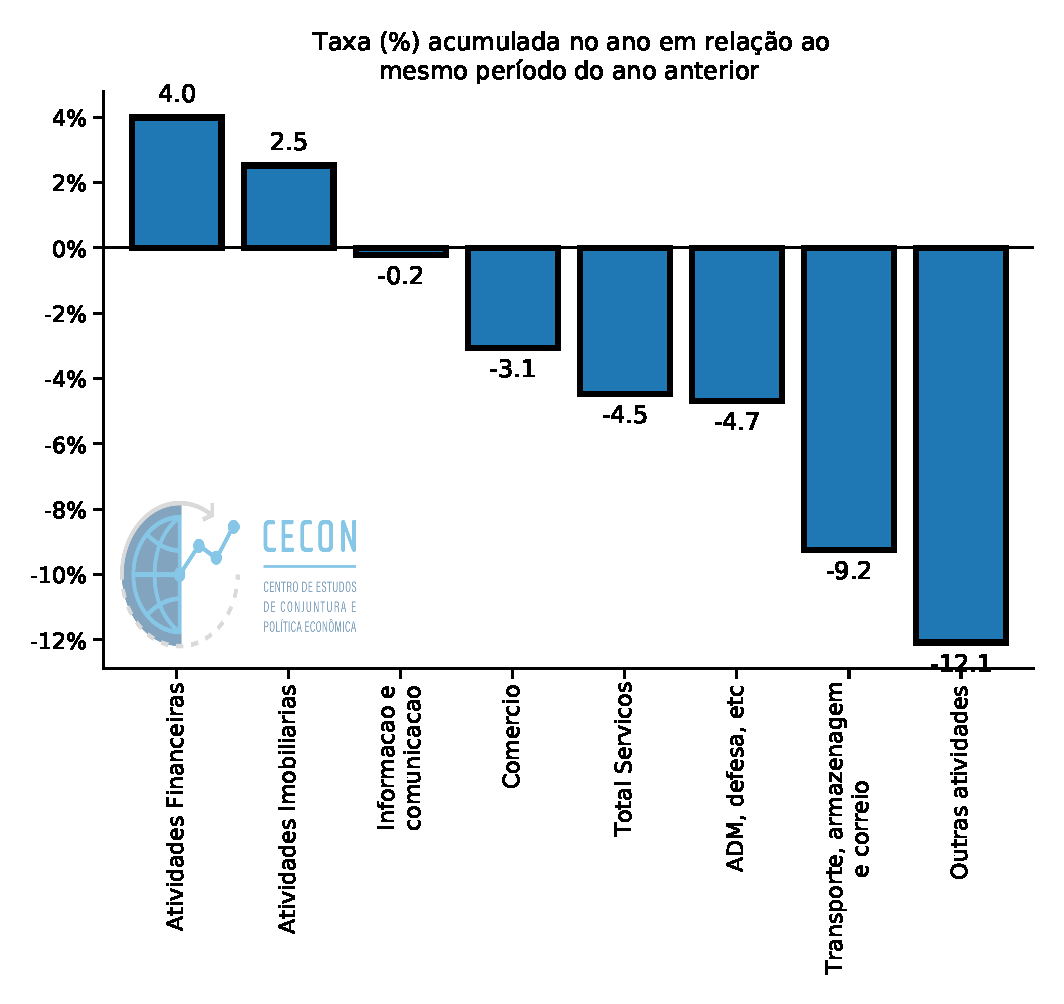
\includegraphics[width=.9\linewidth]{./figs/PIB/Servicos_Acum.pdf}
\end{center}

\subsubsection*{Serviços (comparação com ano anterior)}
\label{sec:orgeeda102}

\begin{center}
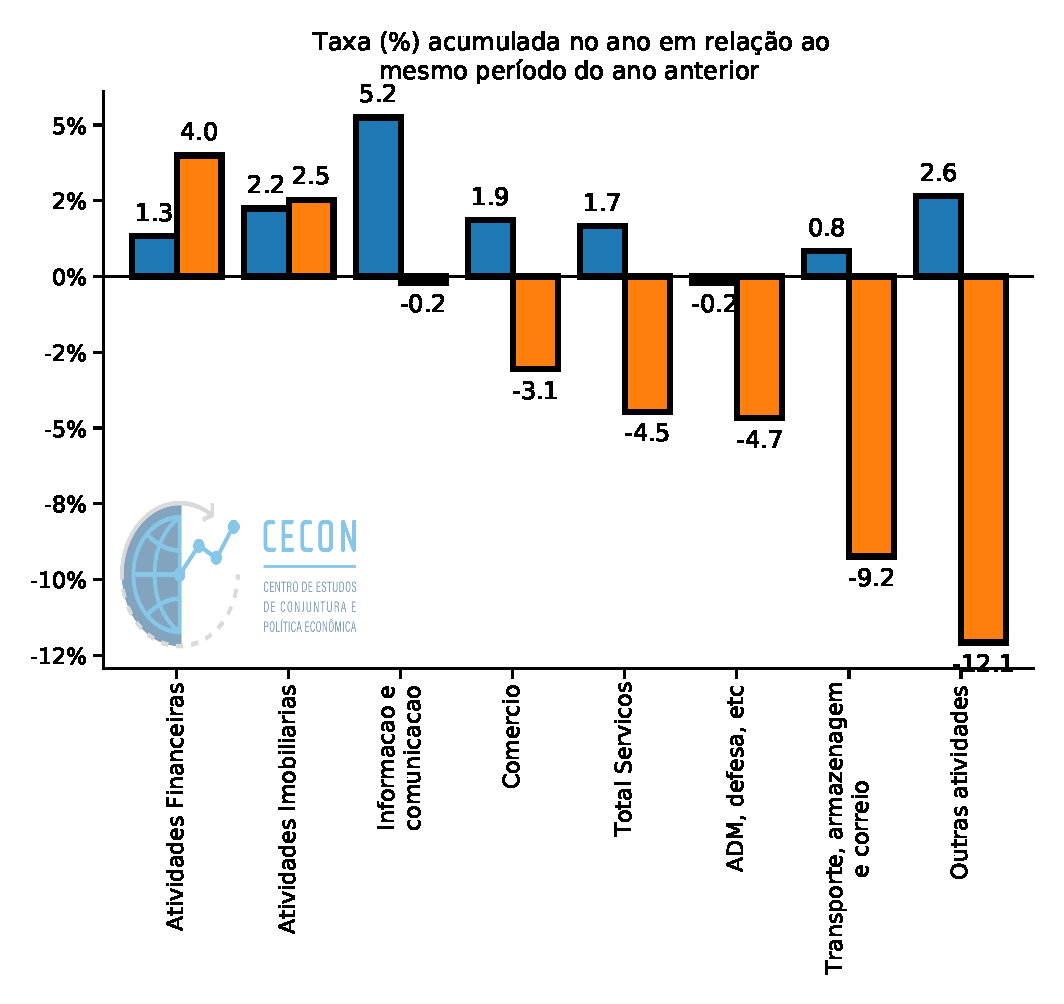
\includegraphics[width=.9\linewidth]{./figs/PIB/Servicos_Acum_Comparativo.pdf}
\end{center}

\subsubsection*{Demanda}
\label{sec:orga7cbba2}

\begin{center}
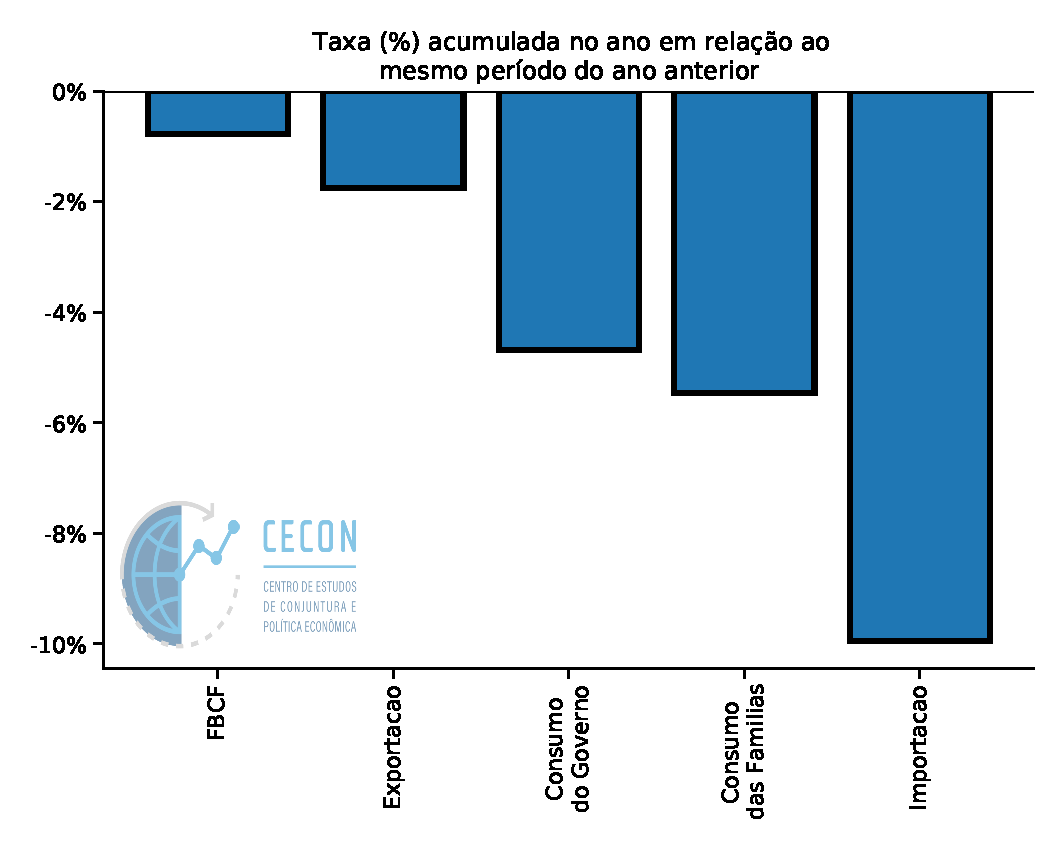
\includegraphics[width=.9\linewidth]{./figs/PIB/Demanda_Acum.pdf}
\end{center}

\subsubsection*{Demanda (comparação com ano anterior)}
\label{sec:org1589aba}

\begin{center}
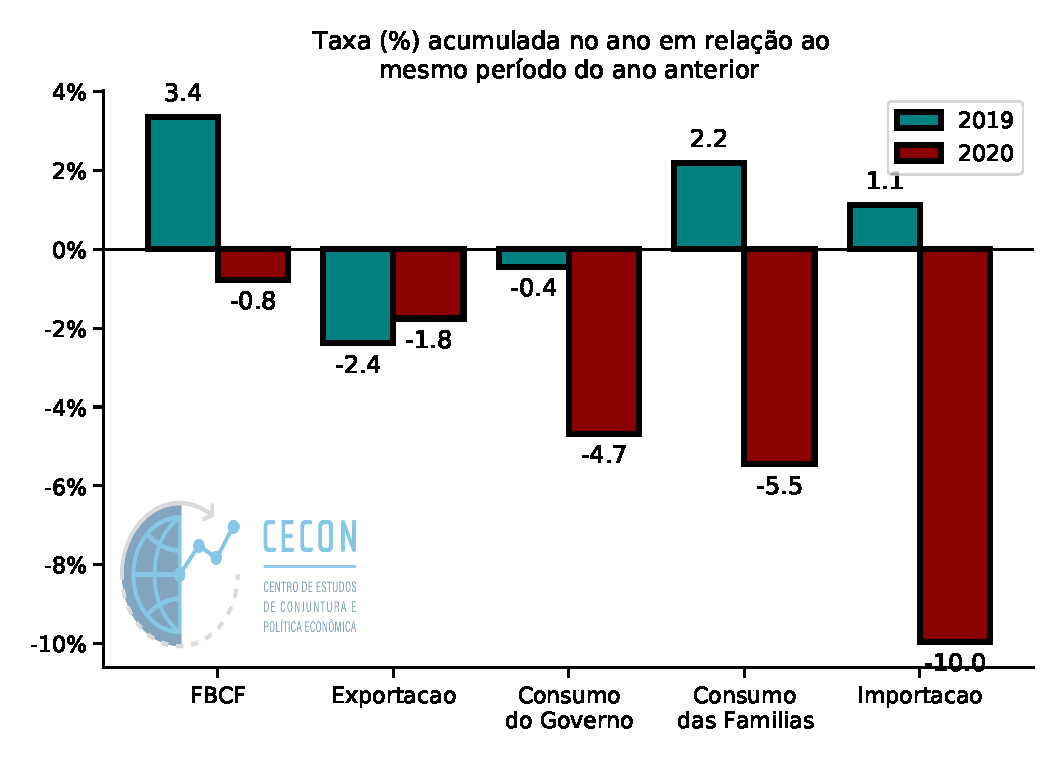
\includegraphics[width=.9\linewidth]{./figs/PIB/Demanda_Acum_Comparativo.pdf}
\end{center}

\subsubsection*{PIB}
\label{sec:org2be222b}

\begin{center}
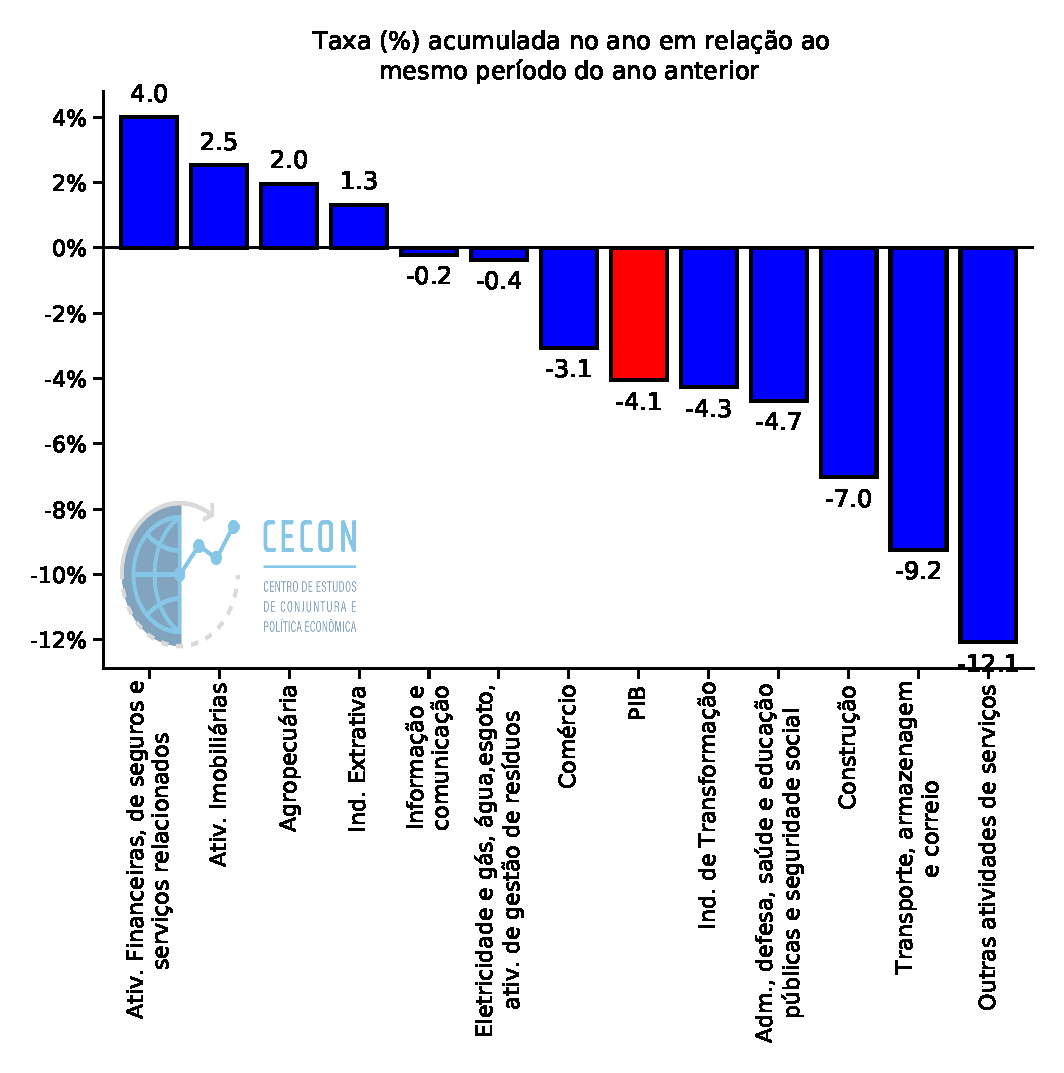
\includegraphics[width=.9\linewidth]{./figs/PIB/PIB_Acum.pdf}
\end{center}

\section*{Crédito}
\label{sec:org59fa7f7}

\subsection*{Endividamento das famílias}
\label{sec:org98f5a96}

\begin{center}
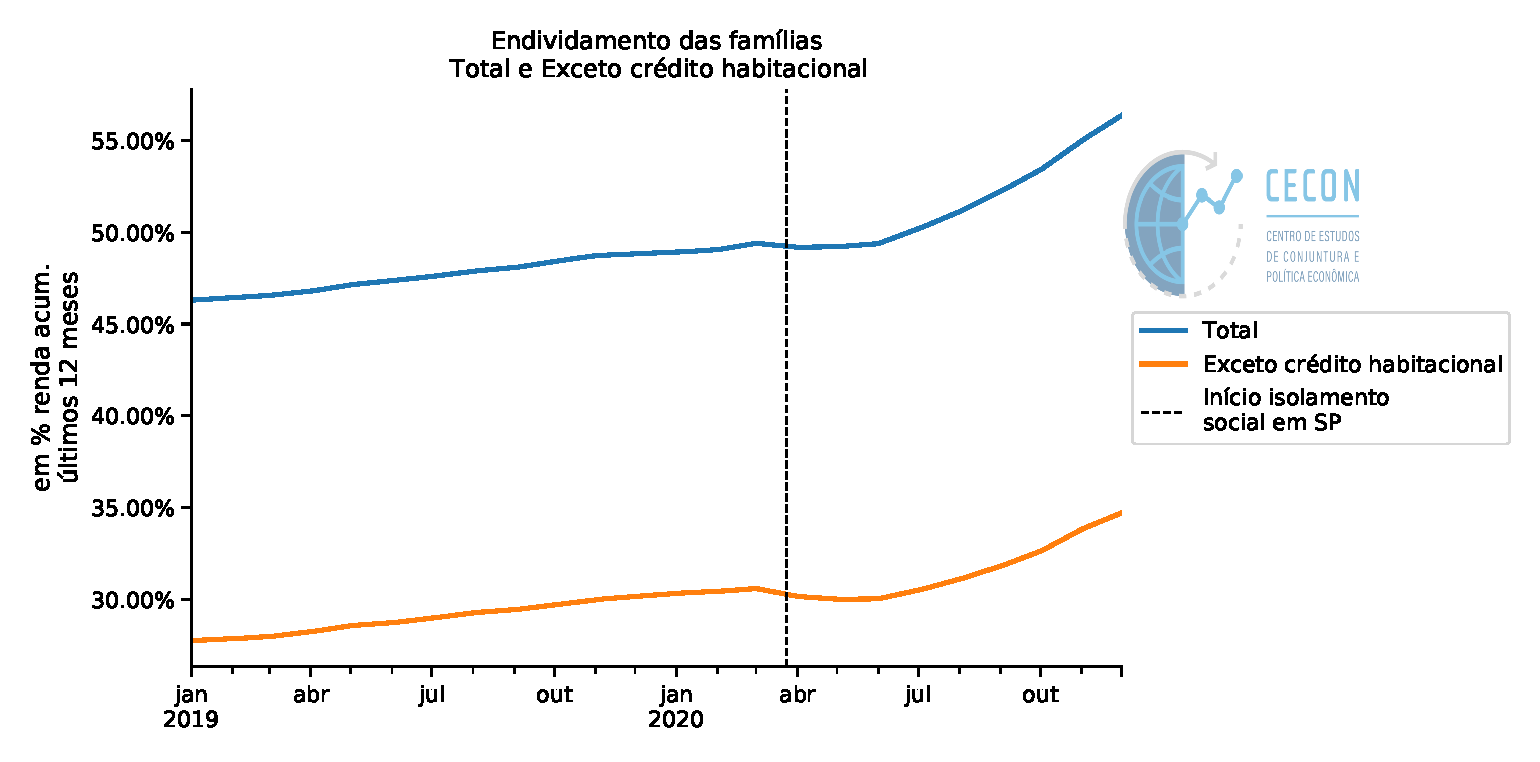
\includegraphics[width=.9\linewidth]{./figs/Credito/EndividamentoFamilias.pdf}
\end{center}


\subsection*{Saldo Pessoal Jurídica - Nível}
\label{sec:org5be84f6}

\begin{center}
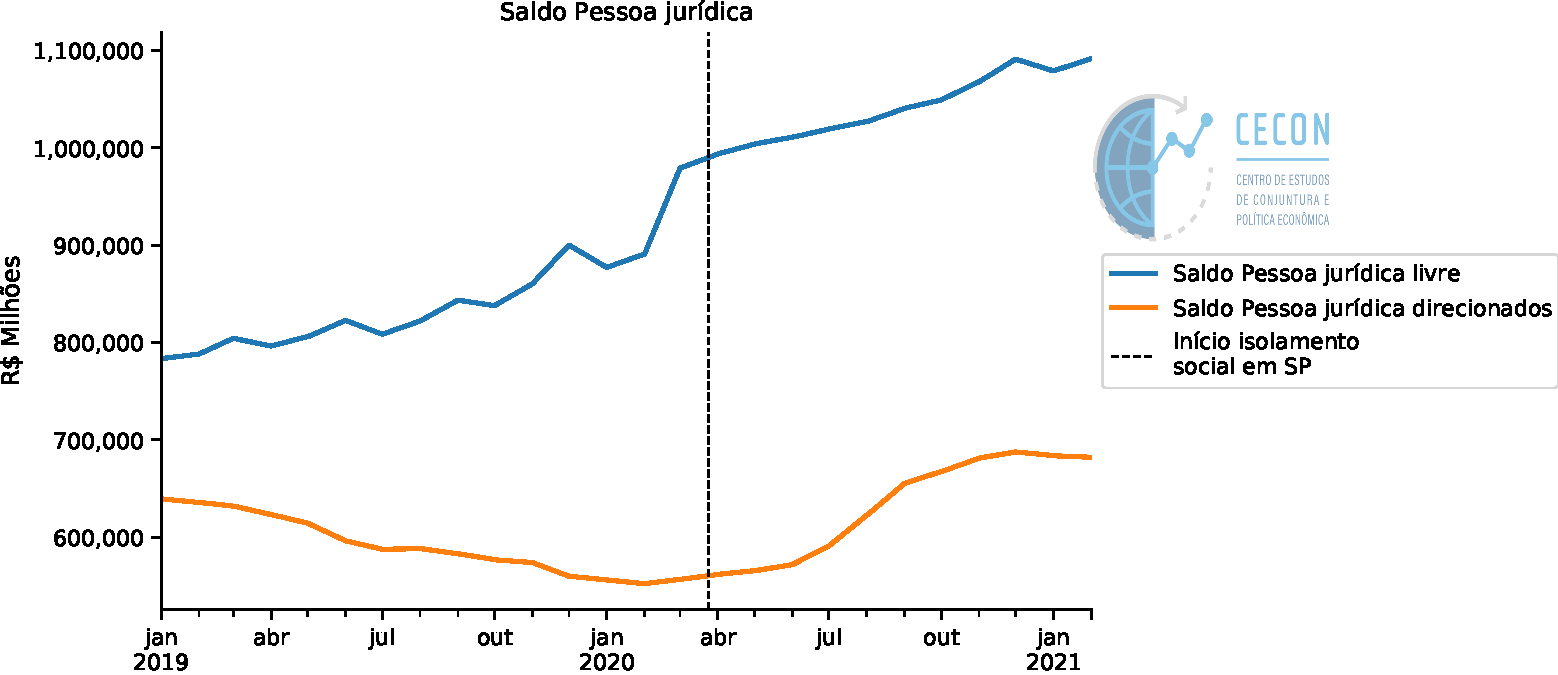
\includegraphics[width=.9\linewidth]{./figs/Credito/SaldoPJ.pdf}
\end{center}



\subsection*{Saldo Pessoa Jurídica - em \% do PIB}
\label{sec:org5a02084}
\begin{center}
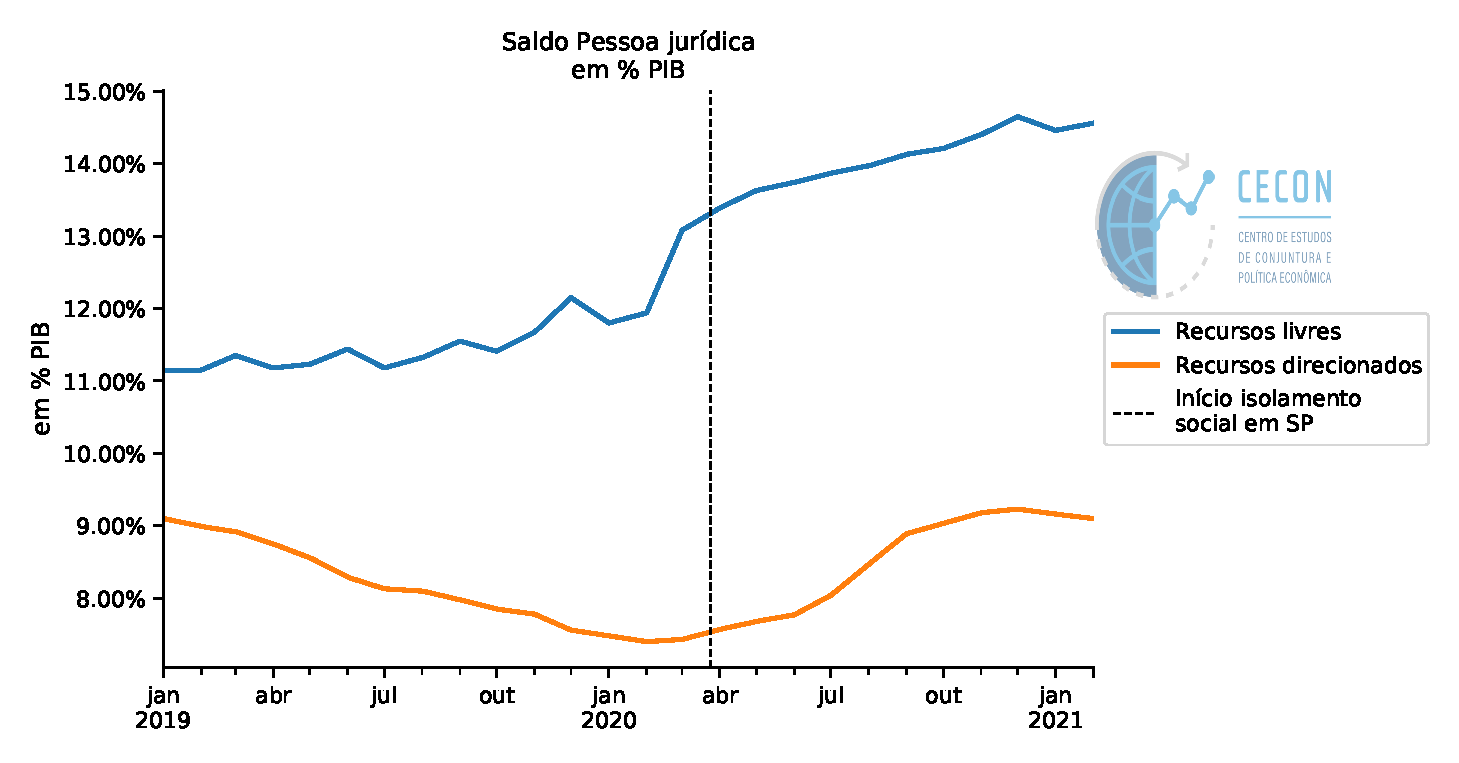
\includegraphics[width=.9\linewidth]{./figs/Credito/SaldoPJ_PIB.pdf}
\end{center}

\subsection*{Saldo Pessoa física - Nível}
\label{sec:org2d74eb7}

\begin{center}
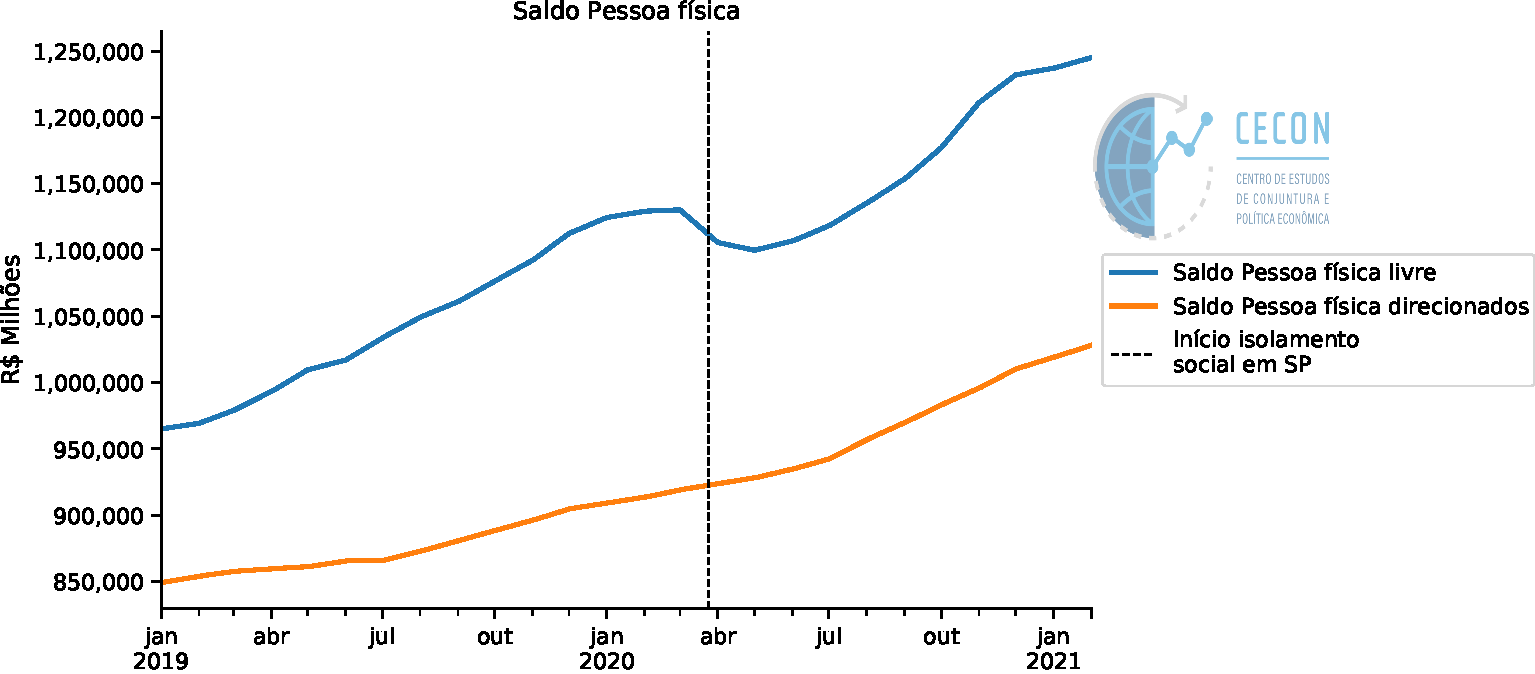
\includegraphics[width=.9\linewidth]{./figs/Credito/SaldoPF.pdf}
\end{center}


\subsection*{Saldo Pessoa física - em \% do PIB}
\label{sec:orgecf9c59}

\begin{center}
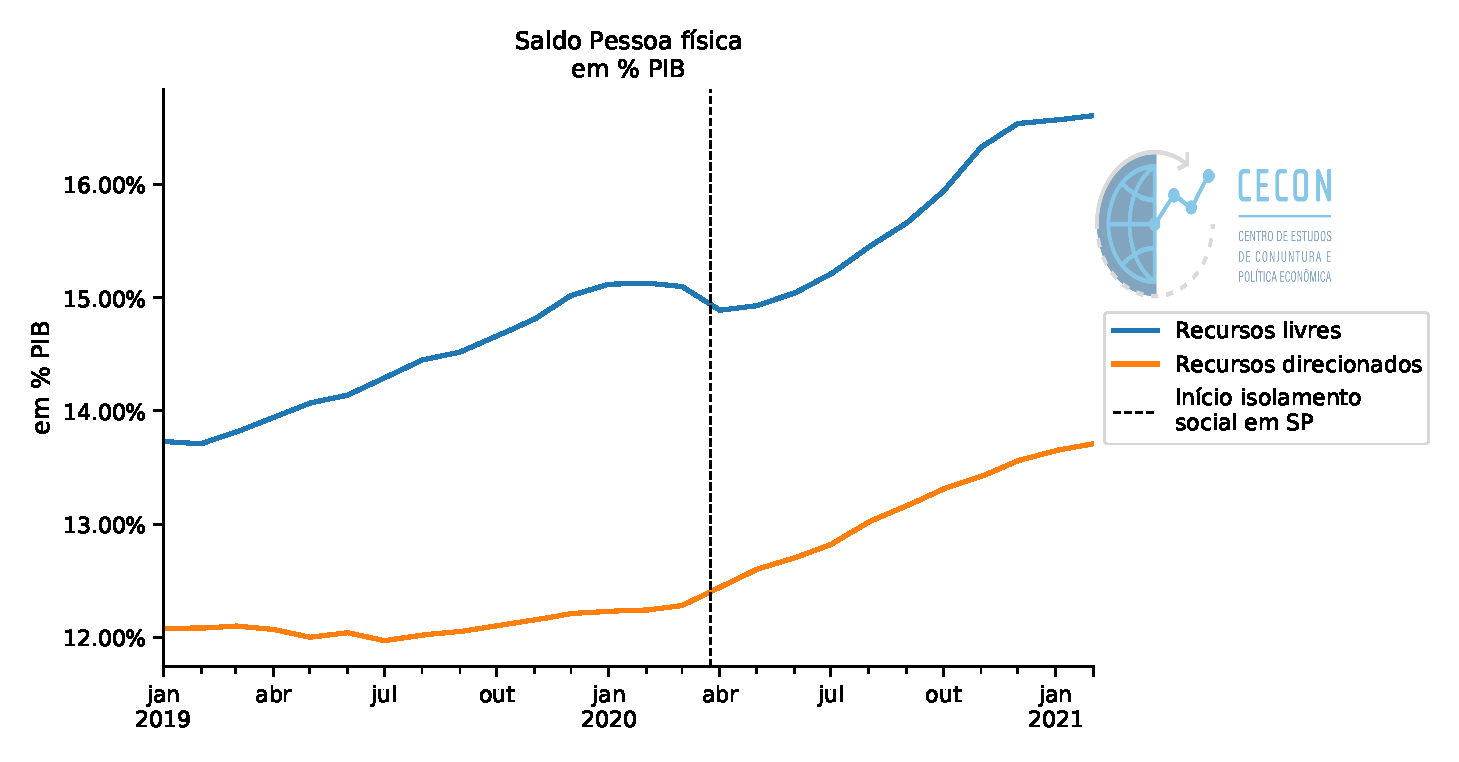
\includegraphics[width=.9\linewidth]{./figs/Credito/SaldoPF_PIB.pdf}
\end{center}


\subsection*{Crédito ampliado em \% do Total}
\label{sec:org3c1407e}

\begin{center}
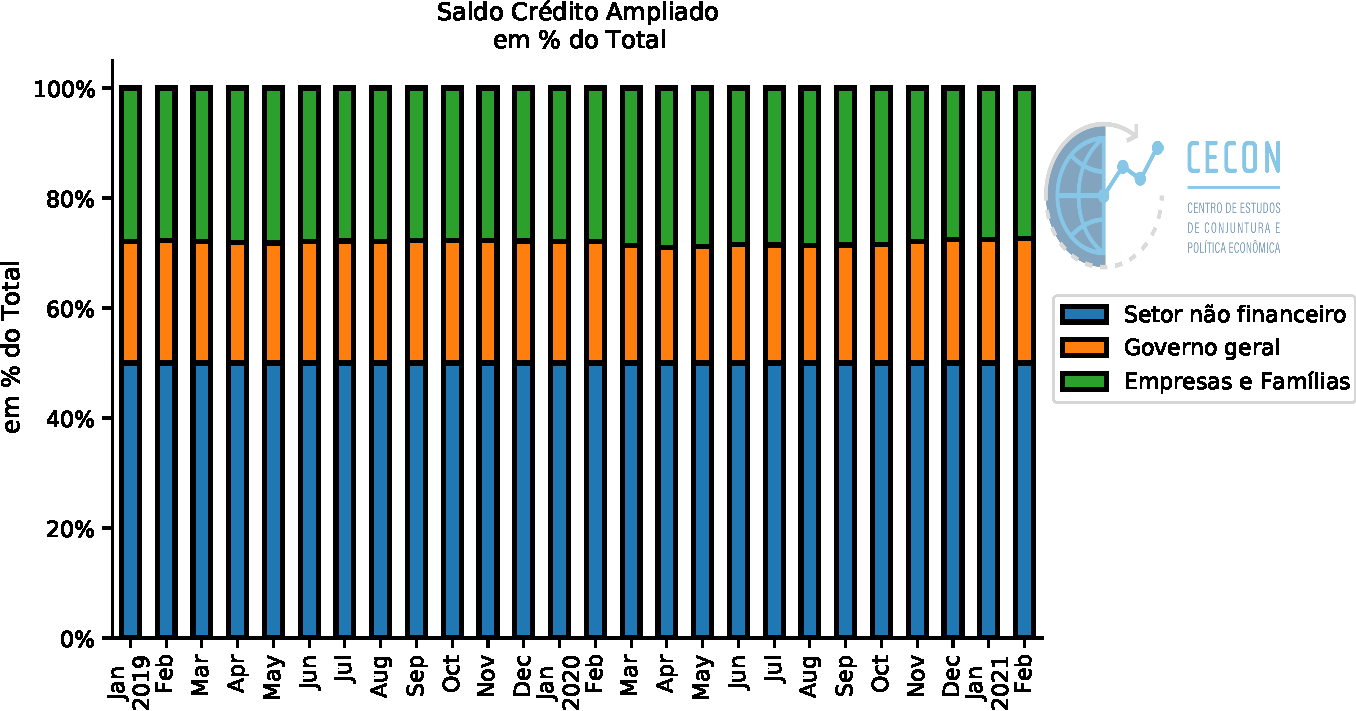
\includegraphics[width=.9\linewidth]{./figs/Credito/SaldoCreditoAmpliado_Total.pdf}
\end{center}

\subsection*{Indicadores de aprovação de crédito}
\label{sec:orga416685}

\begin{center}
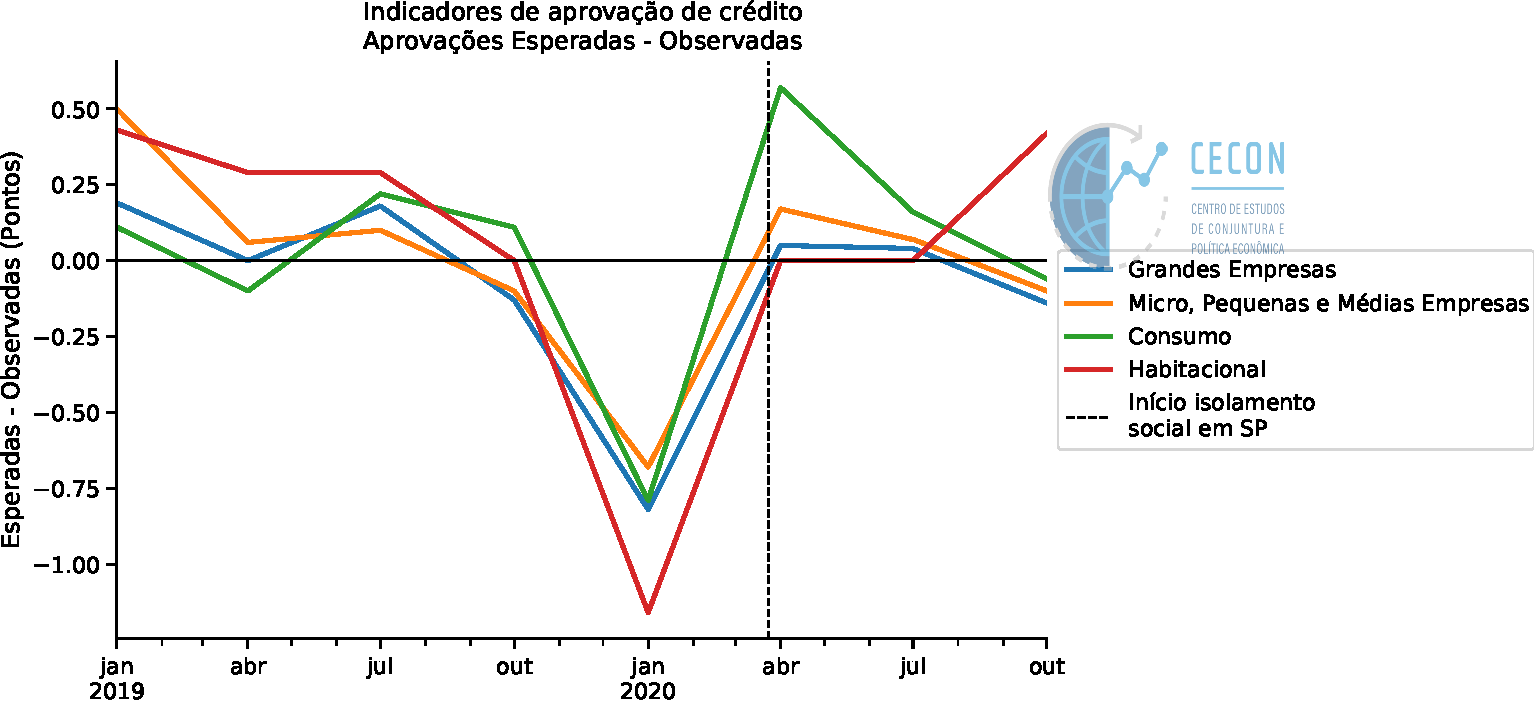
\includegraphics[width=.9\linewidth]{./figs/Credito/PTC.pdf}
\end{center}

\subsection*{Recolhimentos compulsórios de instituições financeiras}
\label{sec:orgd32979e}

\begin{center}
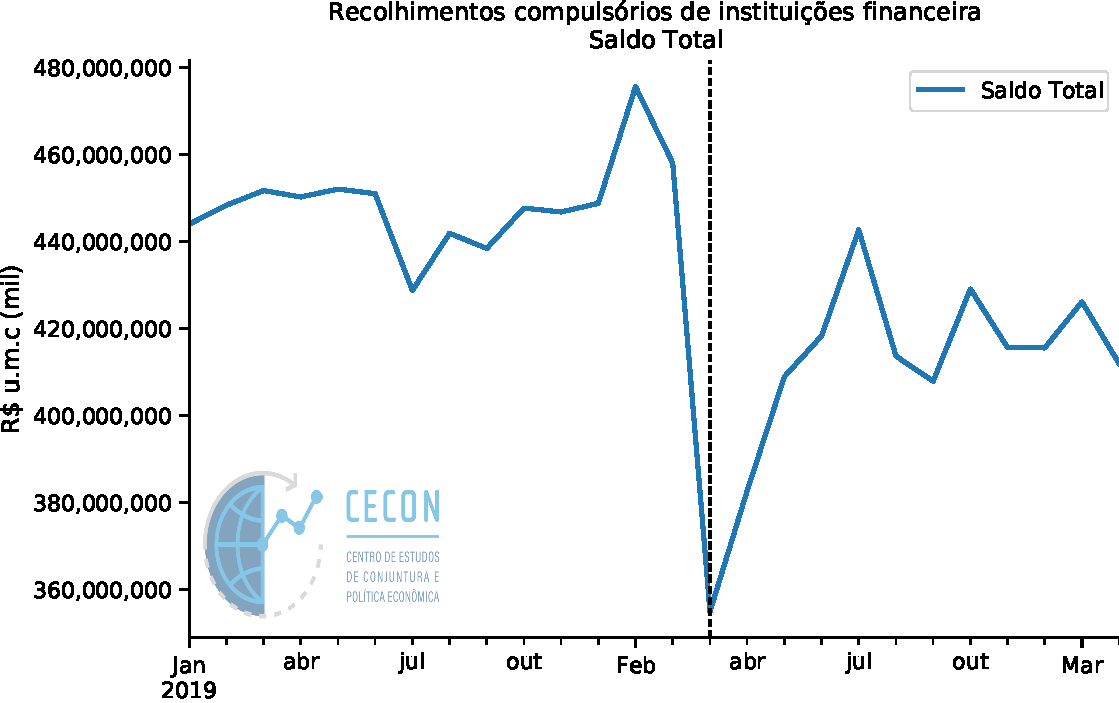
\includegraphics[width=.9\linewidth]{./figs/Credito/Recolhimentos_Total.pdf}
\end{center}

\section*{Índices de atividade setoriais}
\label{sec:org50d8705}


\subsection*{Pesquisa Mensal do Comércio (PMC)}
\label{sec:org641be73}

\begin{center}
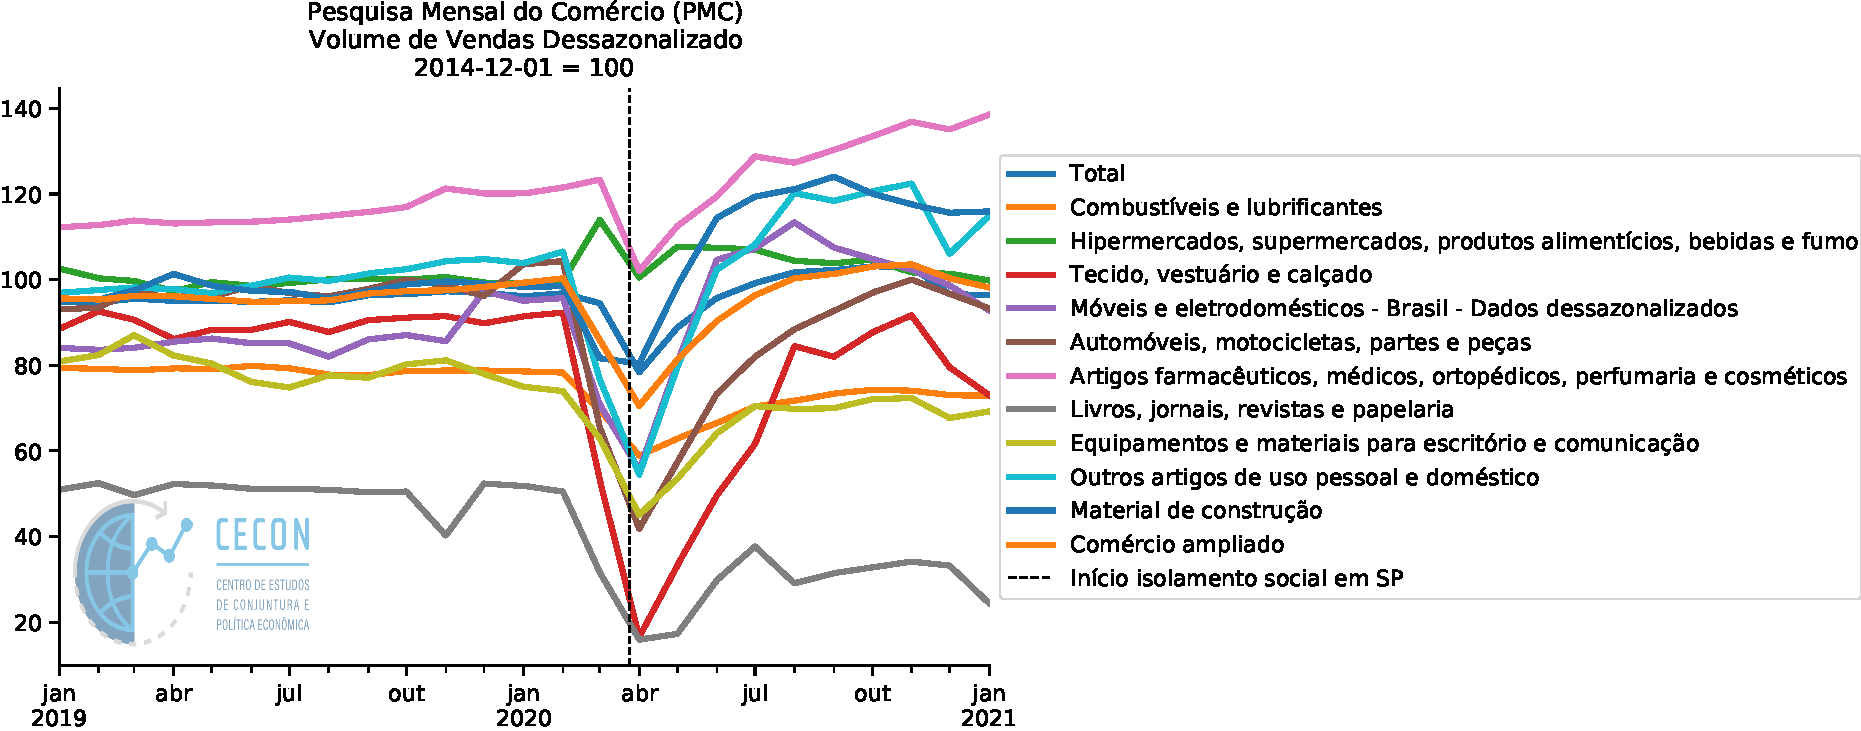
\includegraphics[width=.9\linewidth]{./figs/Setoriais/PMC_IBGE.pdf}
\end{center}


\subsection*{Pesquisa Industrial Mensal (PIM)}
\label{sec:org5848320}

\begin{center}
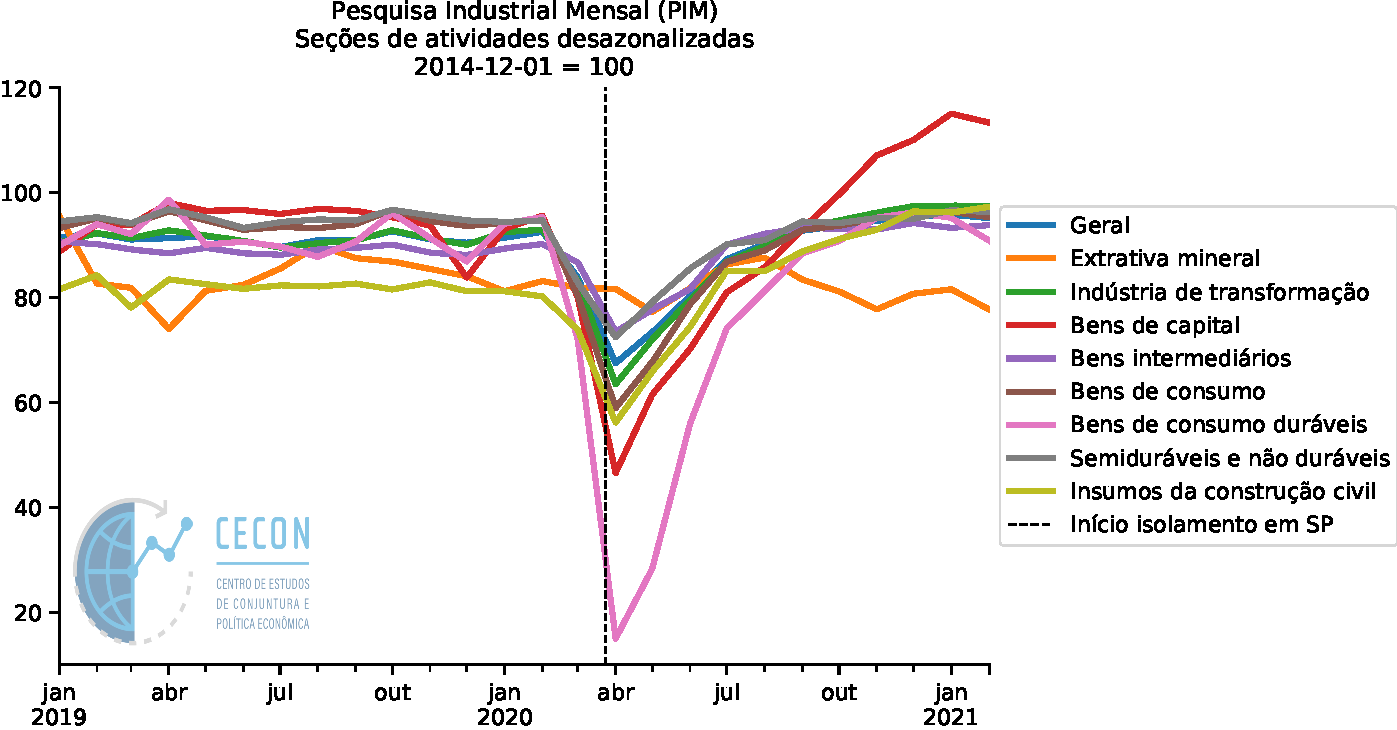
\includegraphics[width=.9\linewidth]{./figs/Setoriais/PIM_IBGE.pdf}
\end{center}


\subsection*{Pesquisa Mensal de Serviços (PMS)}
\label{sec:org314749e}
\subsubsection*{Receita nominal sem ajuste sazonal}
\label{sec:org797f0a9}
\begin{center}
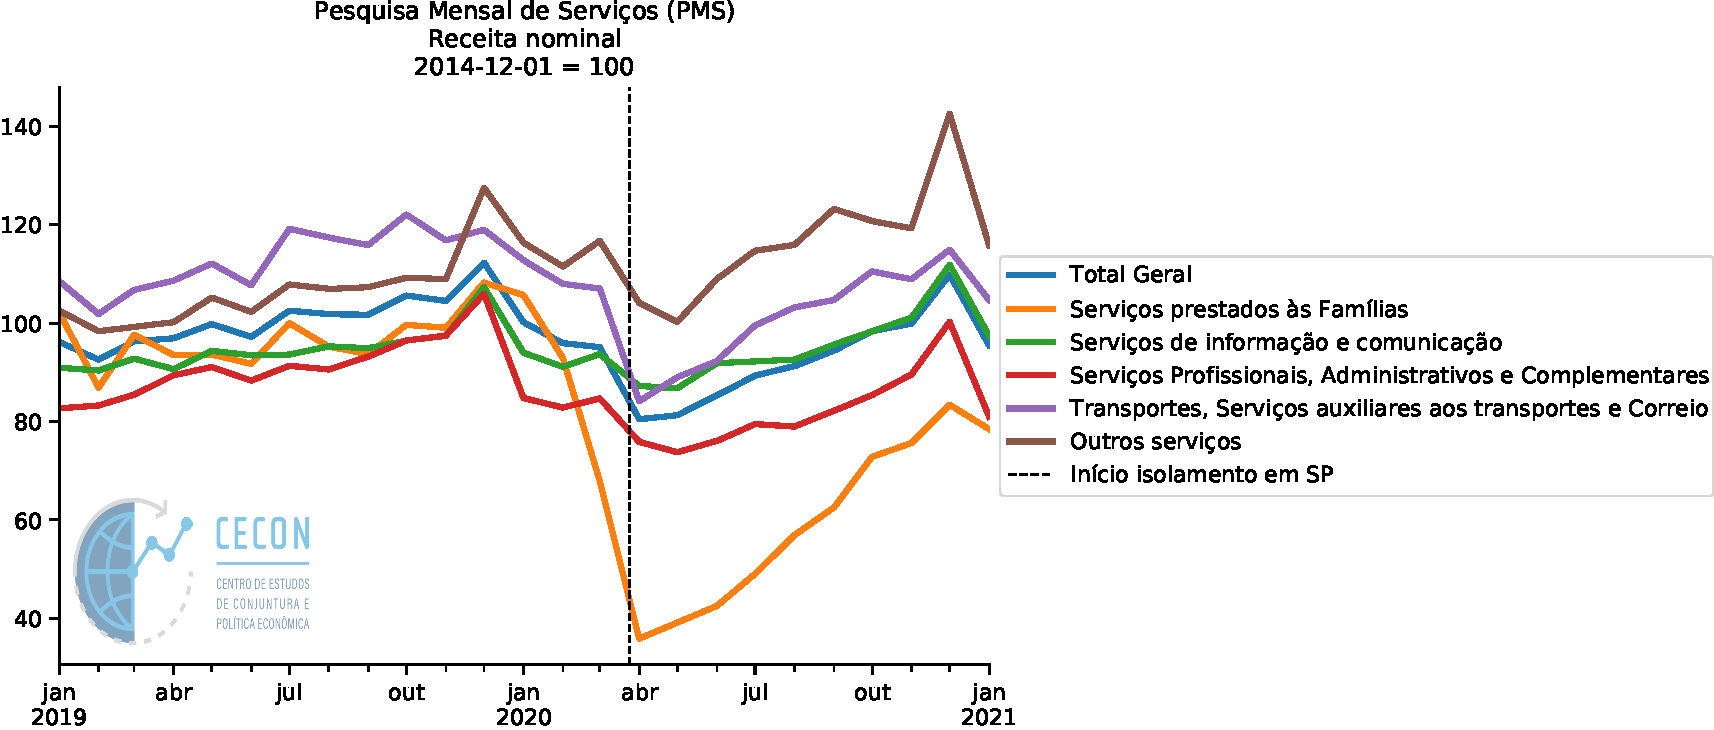
\includegraphics[width=.9\linewidth]{./figs/Setoriais/PMS_IBGE.pdf}
\end{center}

\subsubsection*{Volume com ajuste sazonal}
\label{sec:orgbd8bcbe}


\begin{center}
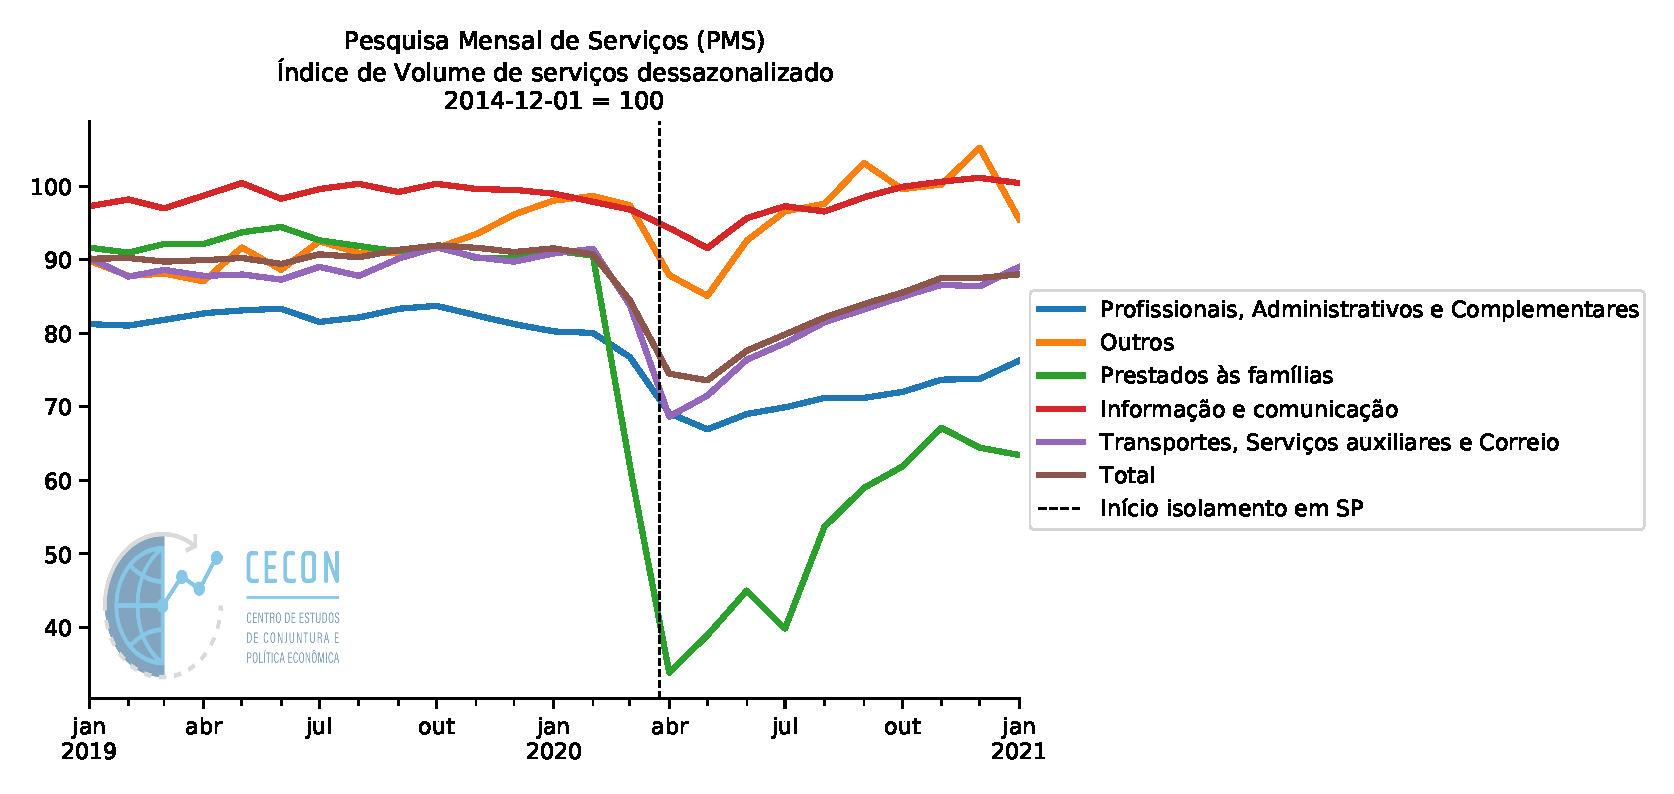
\includegraphics[width=.9\linewidth]{./figs/Setoriais/PMS_vol_dessazonalizada.pdf}
\end{center}

\subsubsection*{Volume com ajuste sazonal (em relação ao mês anterior)}
\label{sec:org902850c}


\begin{center}
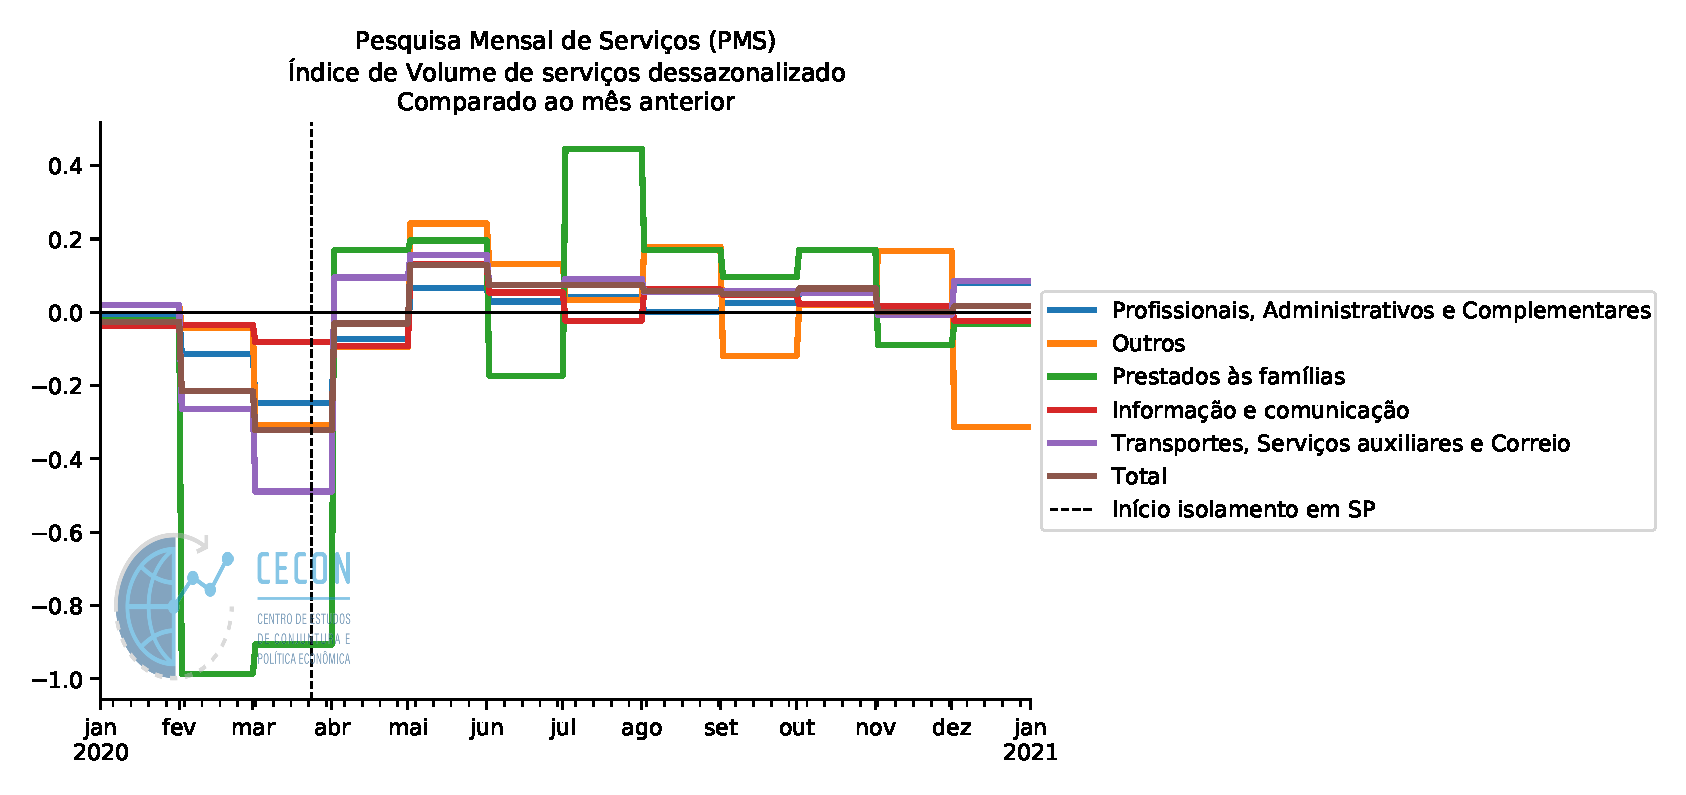
\includegraphics[width=.9\linewidth]{./figs/Setoriais/PMS_vol_dessazonalizada_diff.pdf}
\end{center}

\section*{Emprego}
\label{sec:org8f38a93}

\subsection*{Rendimento médio real habitual das pessoas ocupadas}
\label{sec:org9e5d903}


\begin{center}
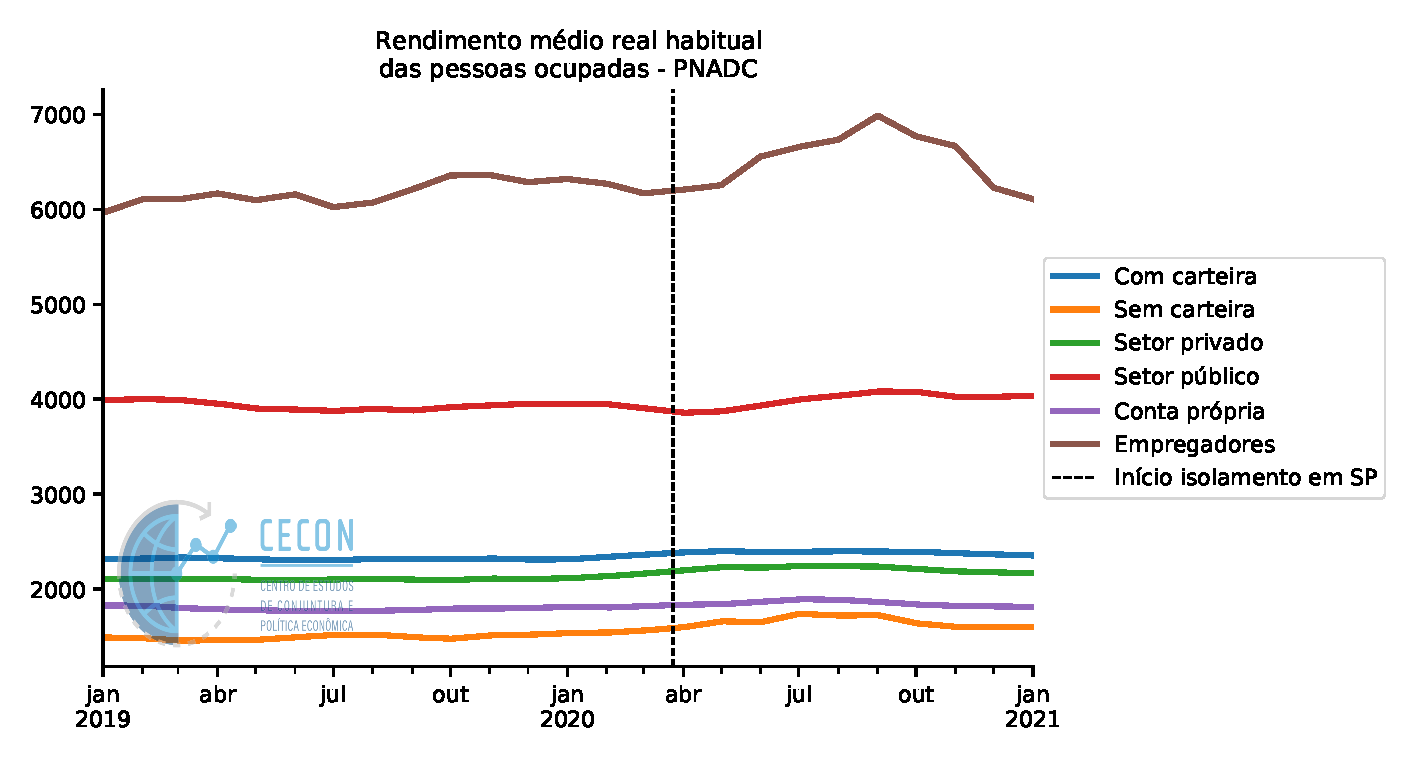
\includegraphics[width=.9\linewidth]{./figs/Emprego/RMHPO.pdf}
\end{center}

\subsection*{Massa de rendimento real efetiva e habitual de todos os trabalhos}
\label{sec:org875888e}

\begin{center}
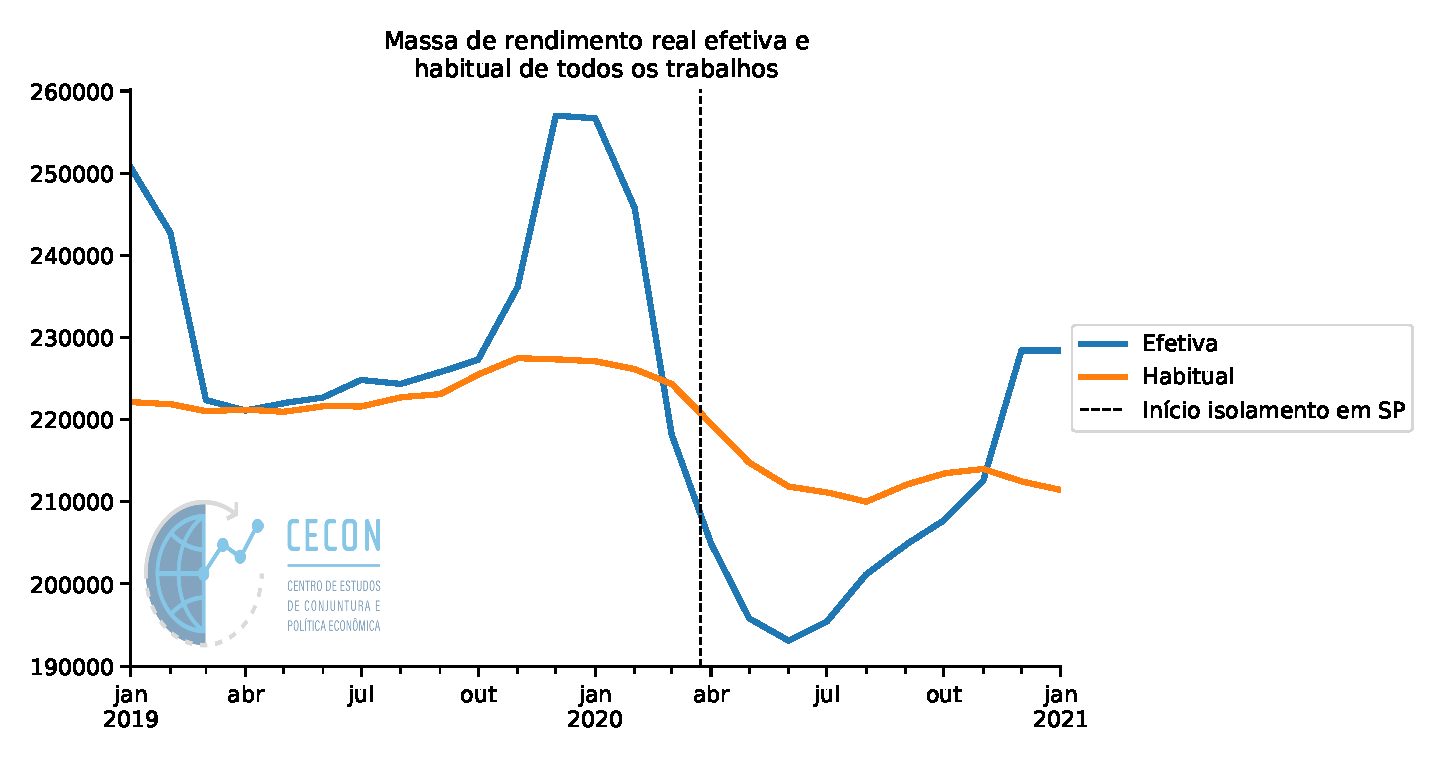
\includegraphics[width=.9\linewidth]{./figs/Emprego/MRR_Efetiva_Habitual.pdf}
\end{center}

\subsection*{Massa Salarial Ampliada Disponível - PNADC}
\label{sec:org68ed89c}

\begin{center}
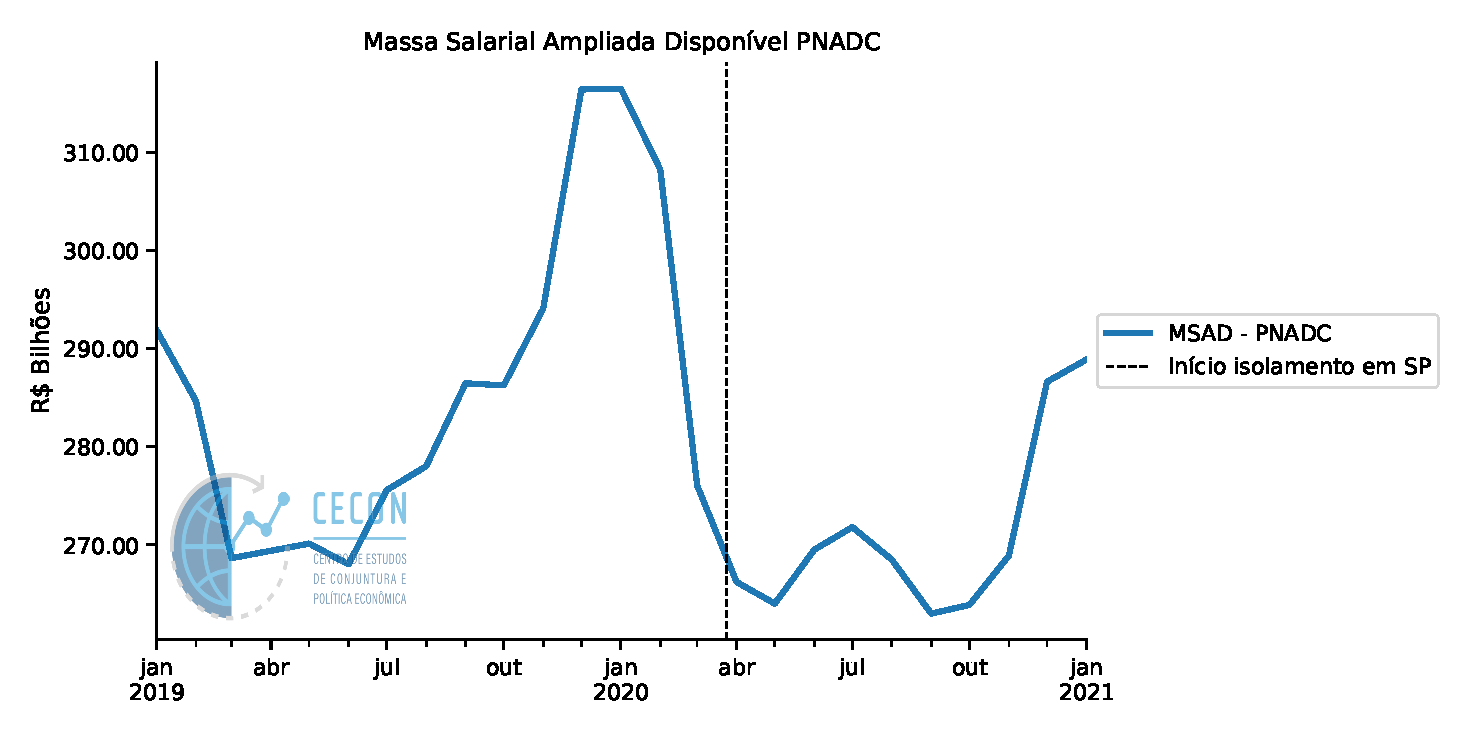
\includegraphics[width=.9\linewidth]{./figs/Emprego/MSAD.pdf}
\end{center}

\subsection*{Rendimento habitual médio por atividade}
\label{sec:org835a232}

\subsection*{Número de horas trabalhadas - indústria de transformação}
\label{sec:org8276d8a}

\begin{center}
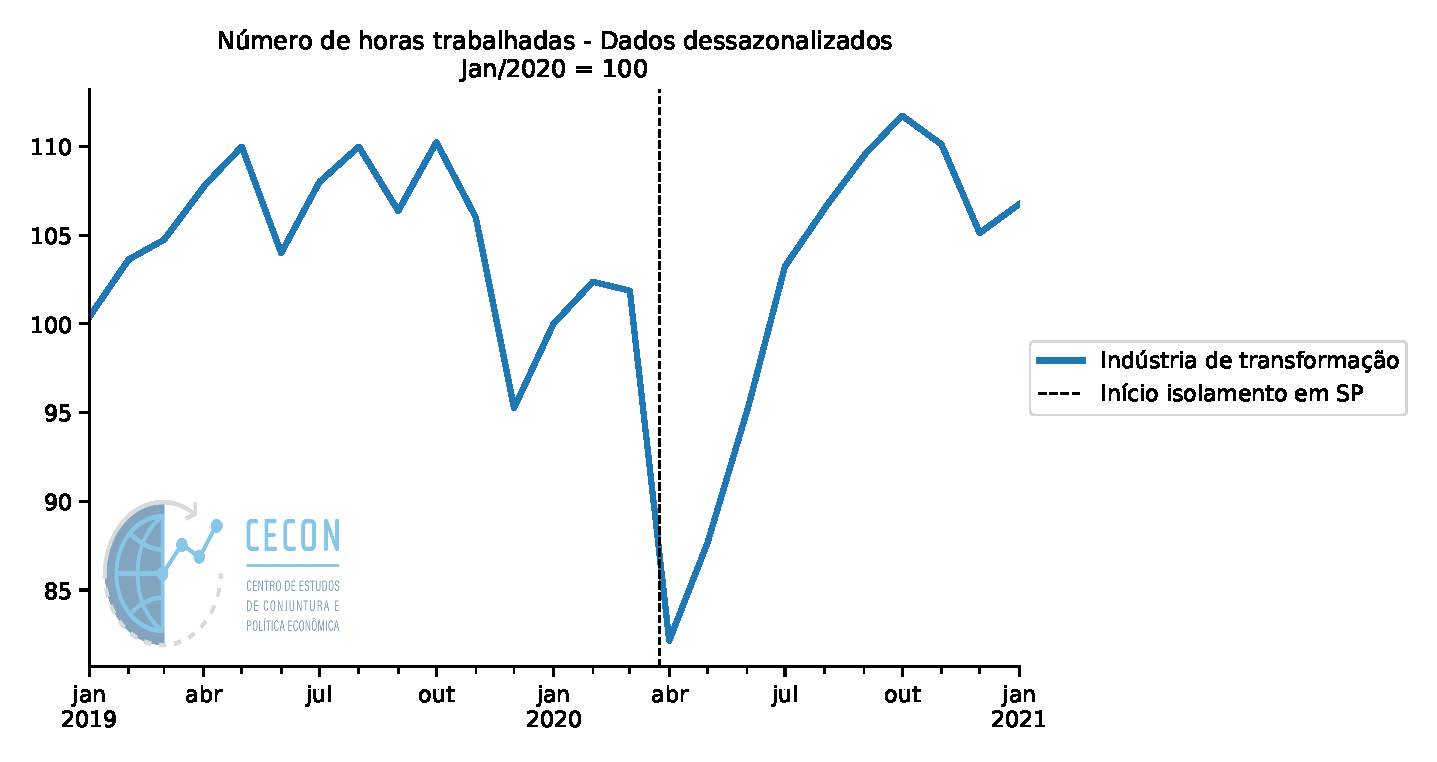
\includegraphics[width=.9\linewidth]{./figs/Emprego/Horas_Transformacao.pdf}
\end{center}

\subsection*{Novo CAGED  - Por atividade (dados dessazonalizados)}
\label{sec:org090a01a}

\begin{center}
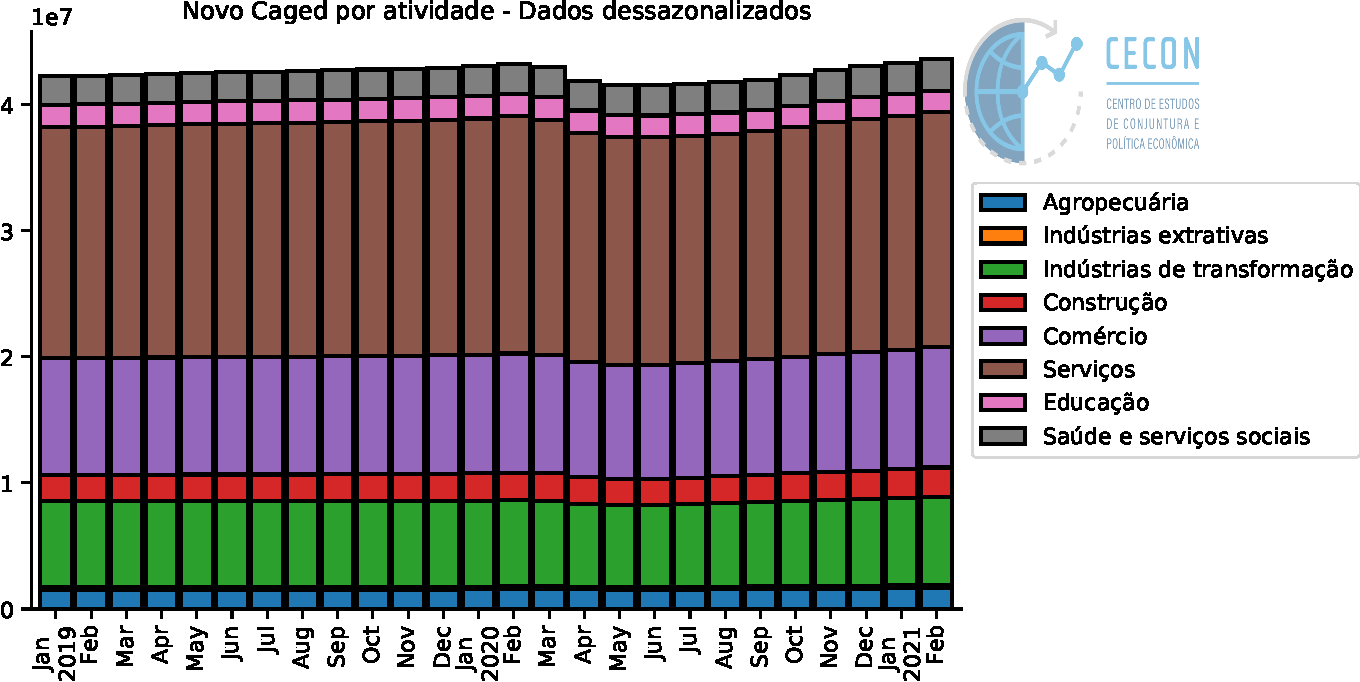
\includegraphics[width=.9\linewidth]{./figs/Emprego/NovoCaged_Atividade.pdf}
\end{center}



\subsection*{Taxa de desocupação}
\label{sec:org771e24e}

\begin{center}
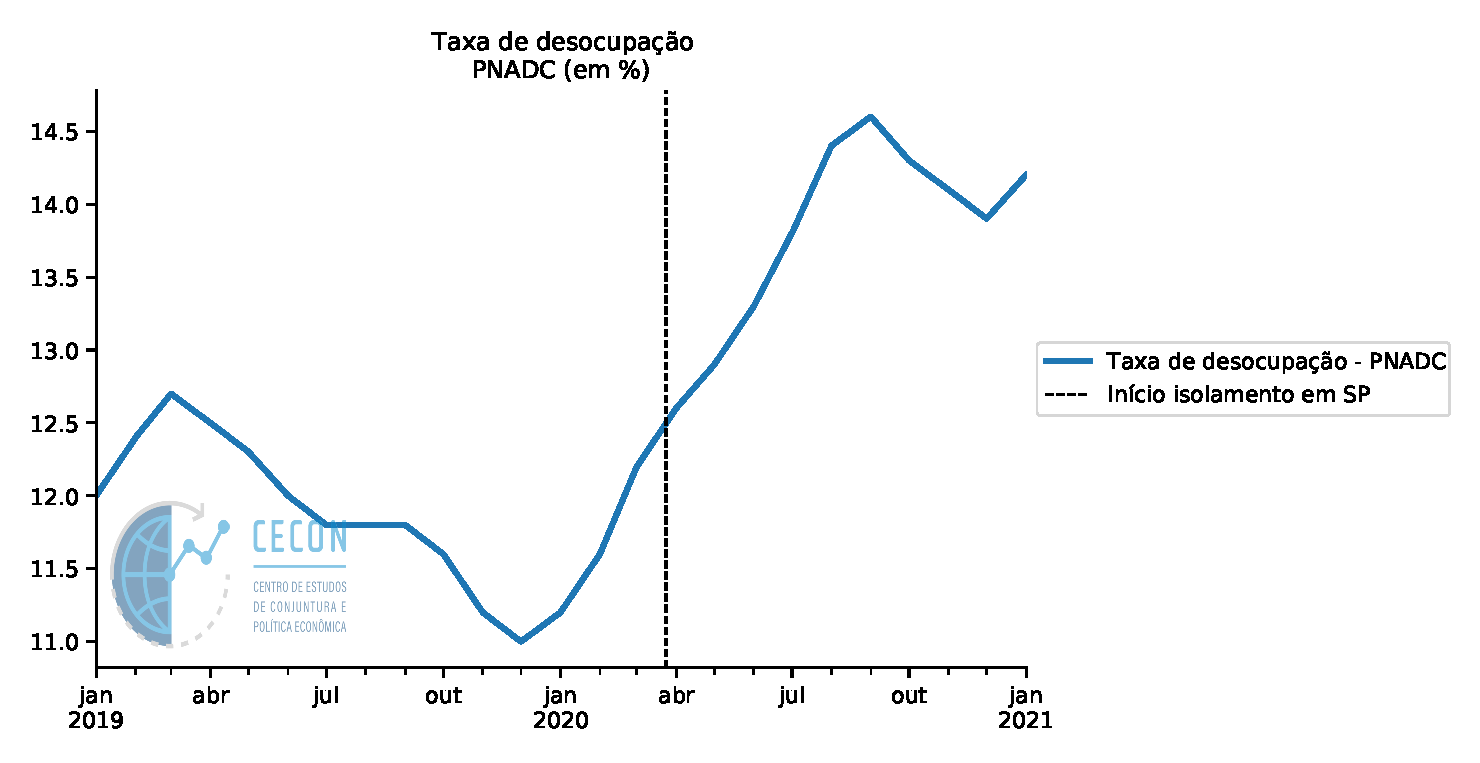
\includegraphics[width=.9\linewidth]{./figs/Emprego/TaxaDesocupacao.pdf}
\end{center}

\section*{PNAD-COVID}
\label{sec:org91ff4d7}
\subsection*{R trial}
\label{sec:orgbc4d201}
\subsection*{Home office - Por sexo e cor}
\label{sec:orgcb6f966}




\begin{center}
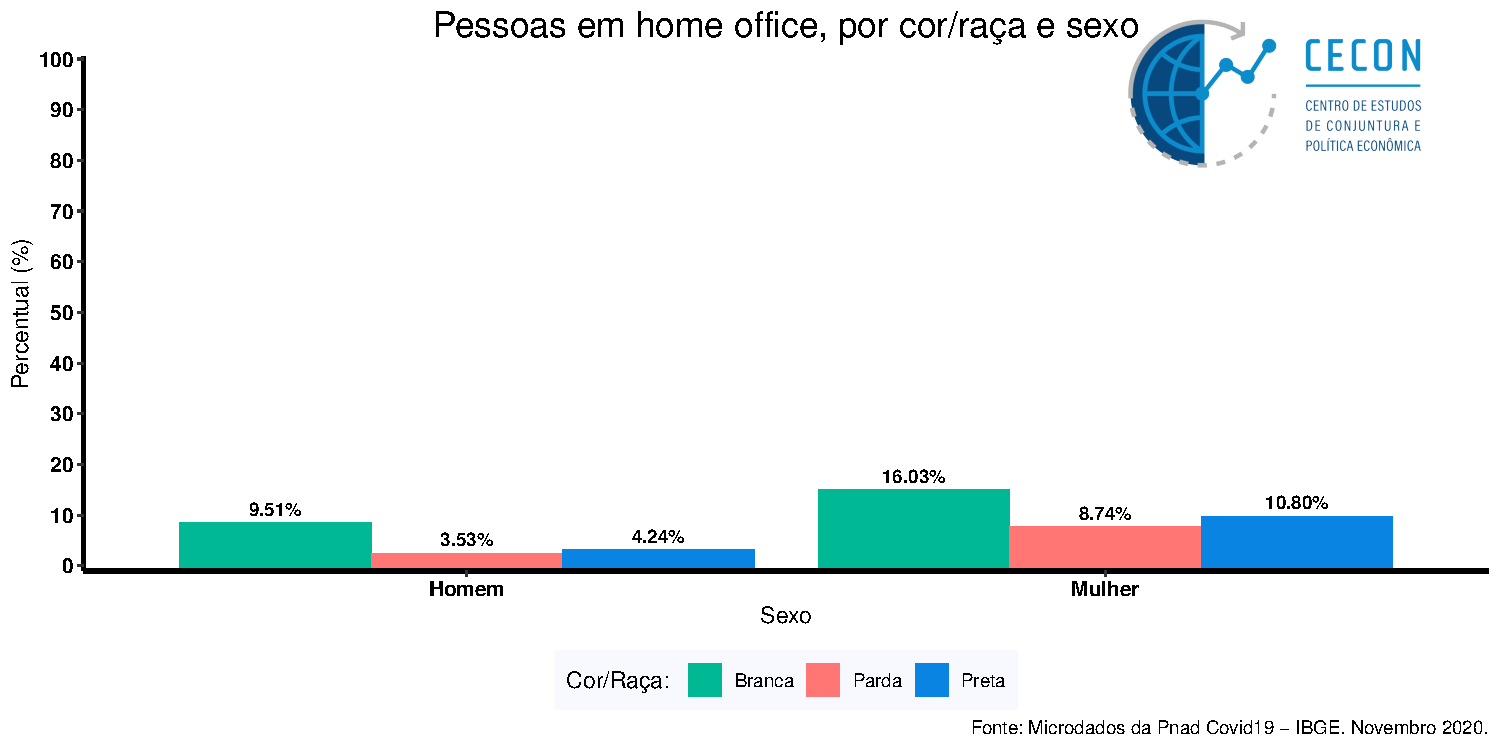
\includegraphics[width=.9\linewidth]{./figs/PNAD_COVID/home_sexo_cor.pdf}
\end{center}

\subsection*{Home office - Por Cor e Escolaridade}
\label{sec:orgaaf3457}
\begin{center}
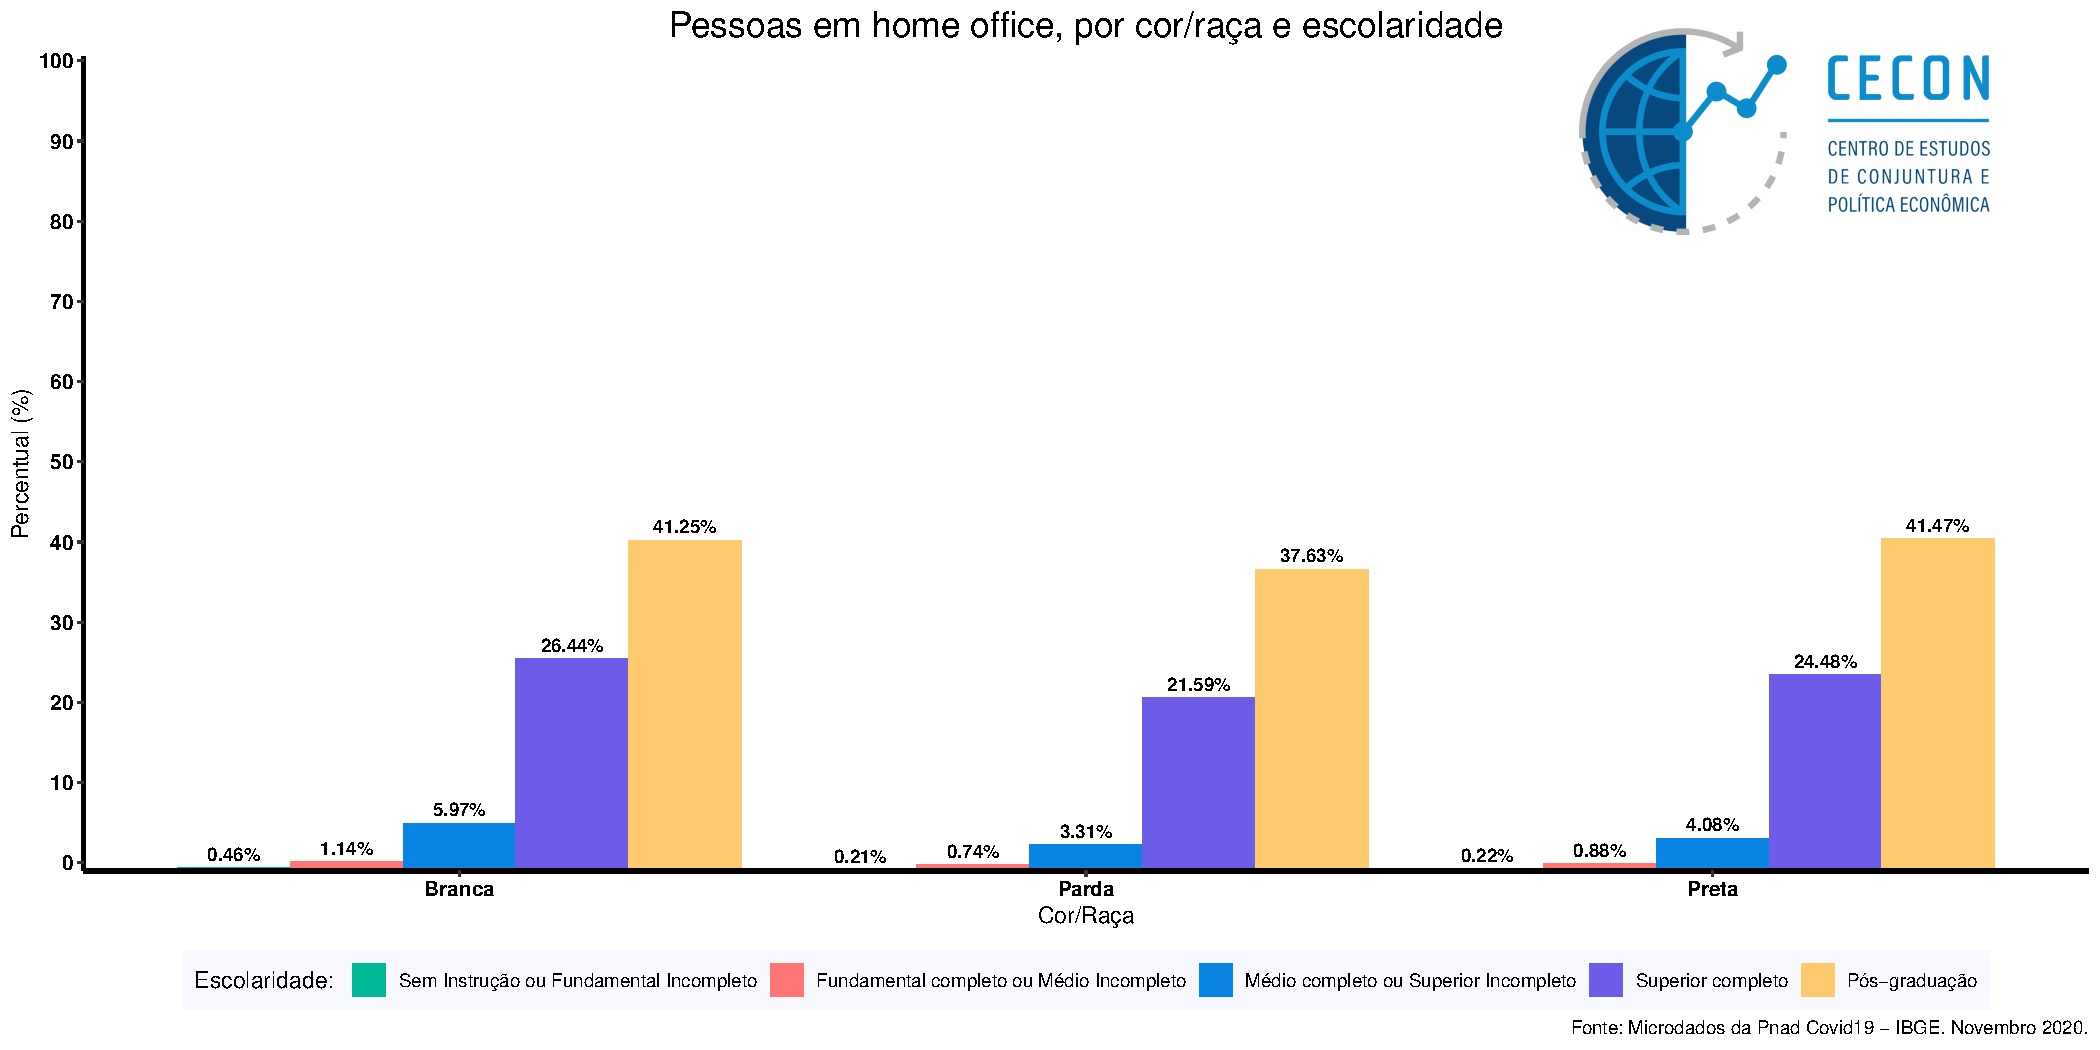
\includegraphics[width=.9\linewidth]{./figs/PNAD_COVID/home_edu_cor.pdf}
\end{center}
\subsection*{Home office - Por Cor e Idade}
\label{sec:org28ef649}
\begin{center}
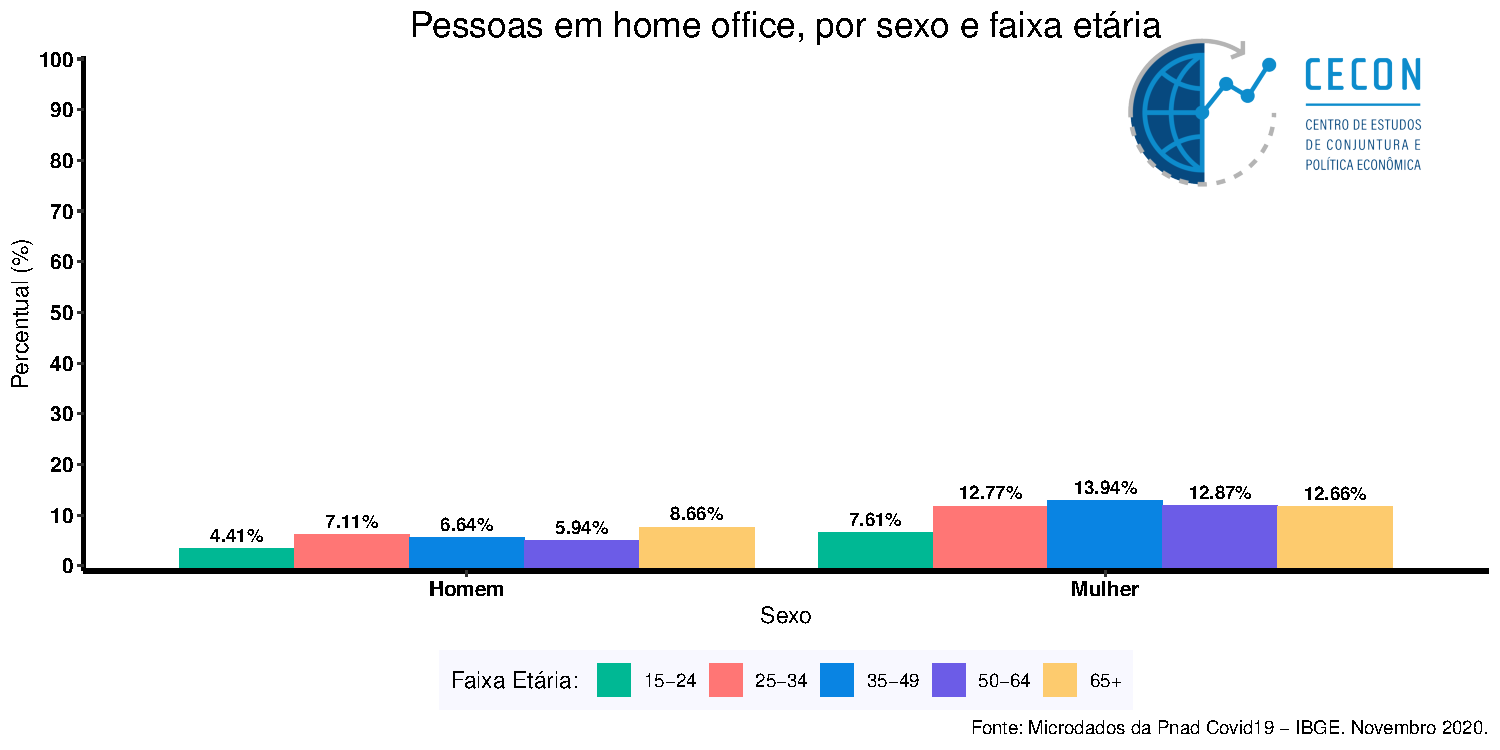
\includegraphics[width=.9\linewidth]{./figs/PNAD_COVID/home_sexo_idade.pdf}
\end{center}

\subsection*{Home office - Por Trabalho}
\label{sec:orgf360caf}
\begin{center}
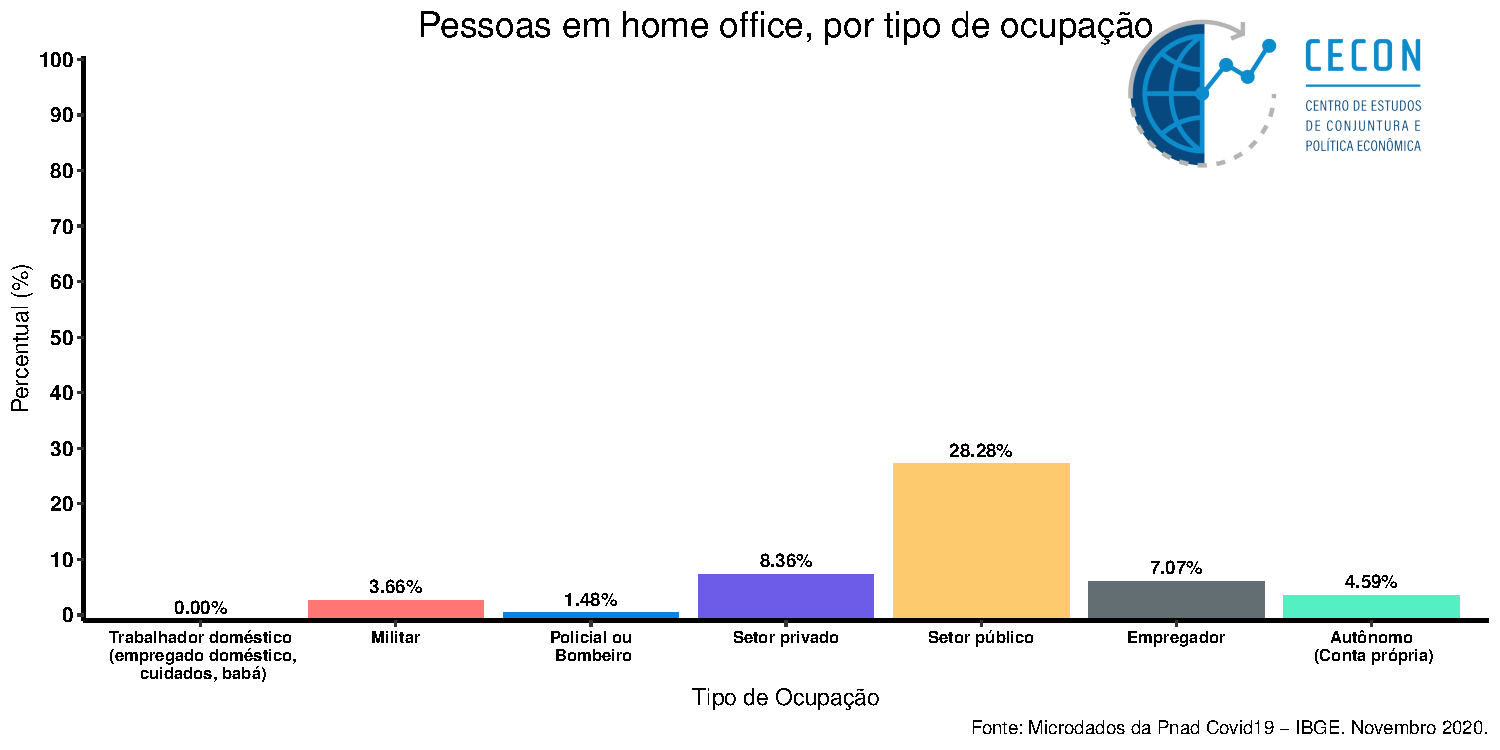
\includegraphics[width=.9\linewidth]{./figs/PNAD_COVID/home_emprego.pdf}
\end{center}

\subsection*{Home office - Por faixa salarial e cor}
\label{sec:orgb39522e}
\begin{center}
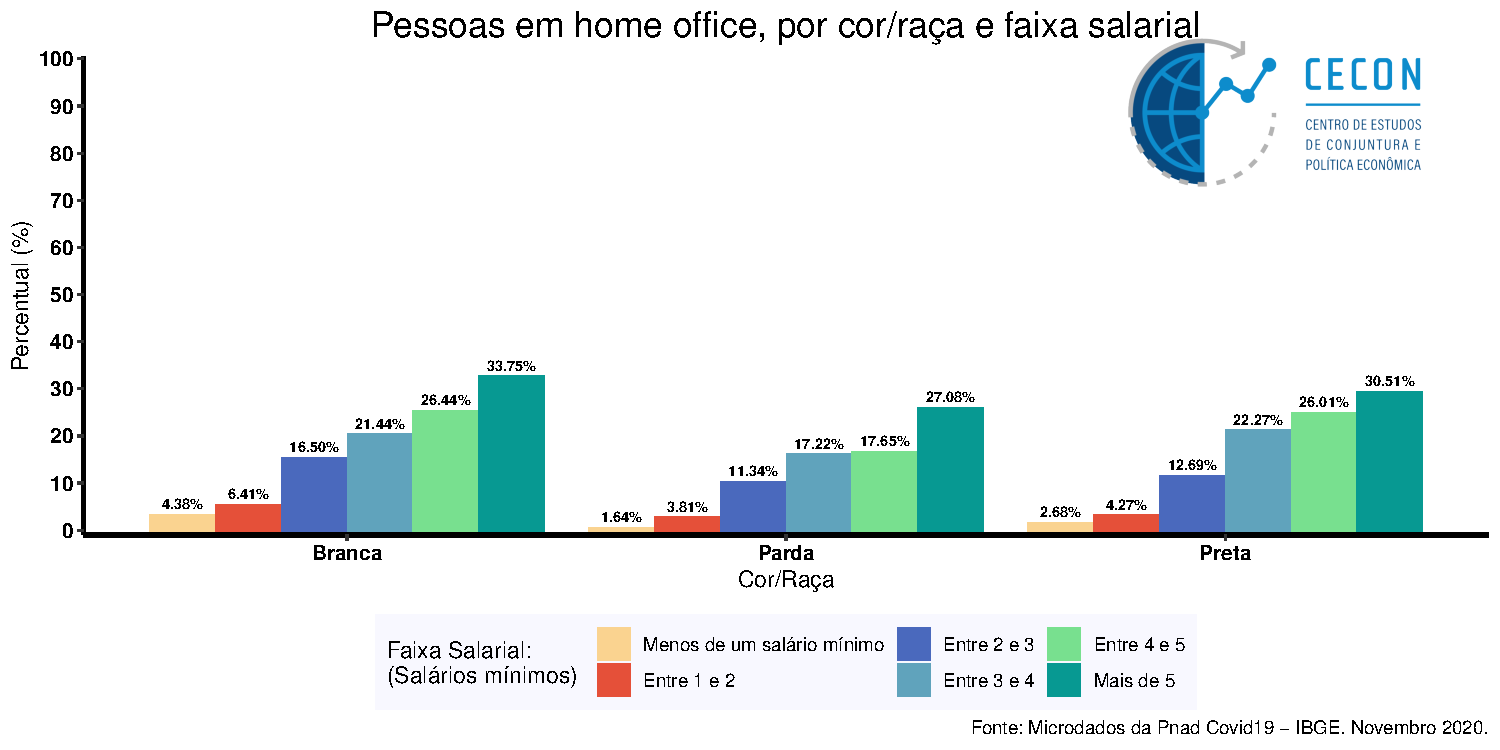
\includegraphics[width=.9\linewidth]{./figs/PNAD_COVID/home_renda.pdf}
\end{center}
\subsection*{Auxilio - Faixa Salarial}
\label{sec:orgf76e355}
\begin{center}
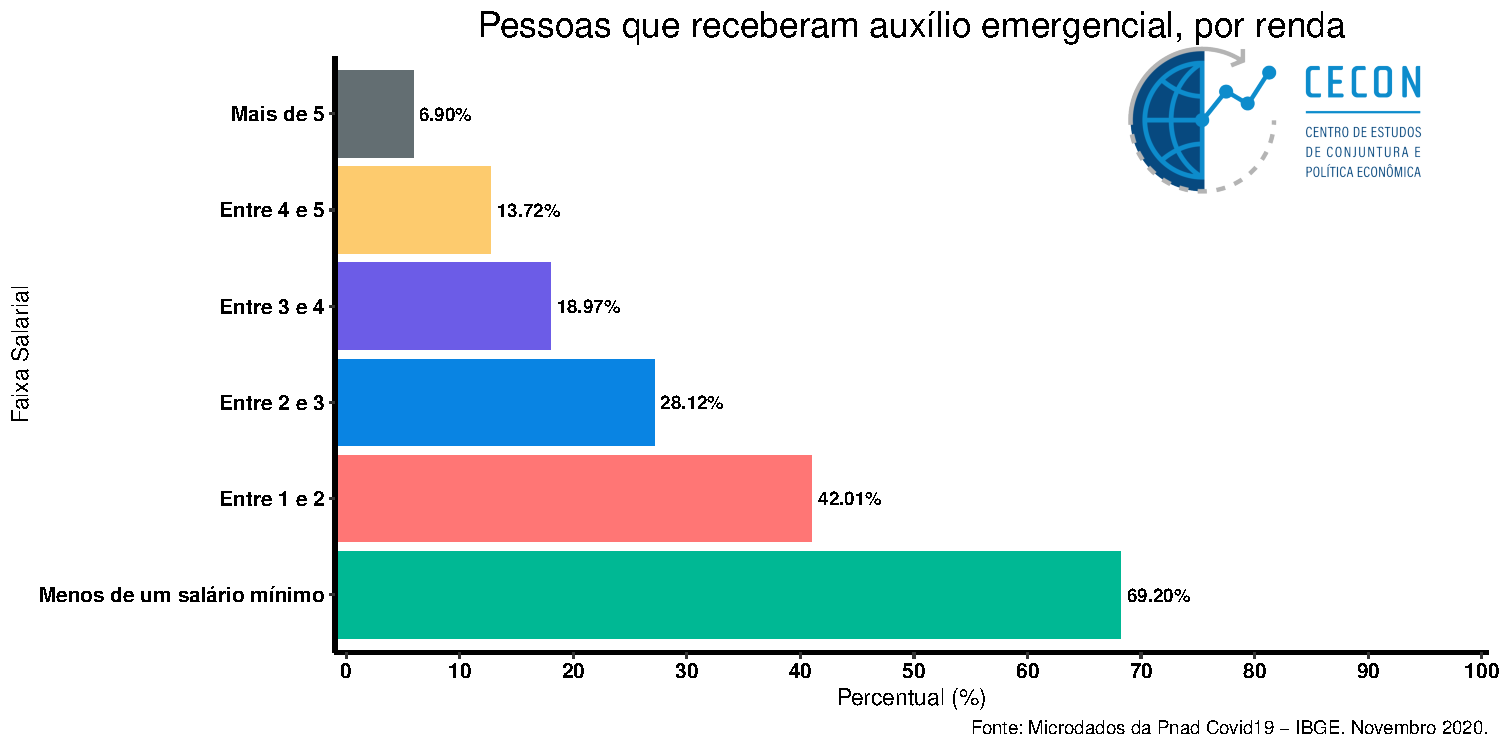
\includegraphics[width=.9\linewidth]{./figs/PNAD_COVID/auxilio_renda.pdf}
\end{center}
\subsection*{Auxilio - Por tipo do domicilio}
\label{sec:orgeaba7ec}
\begin{center}
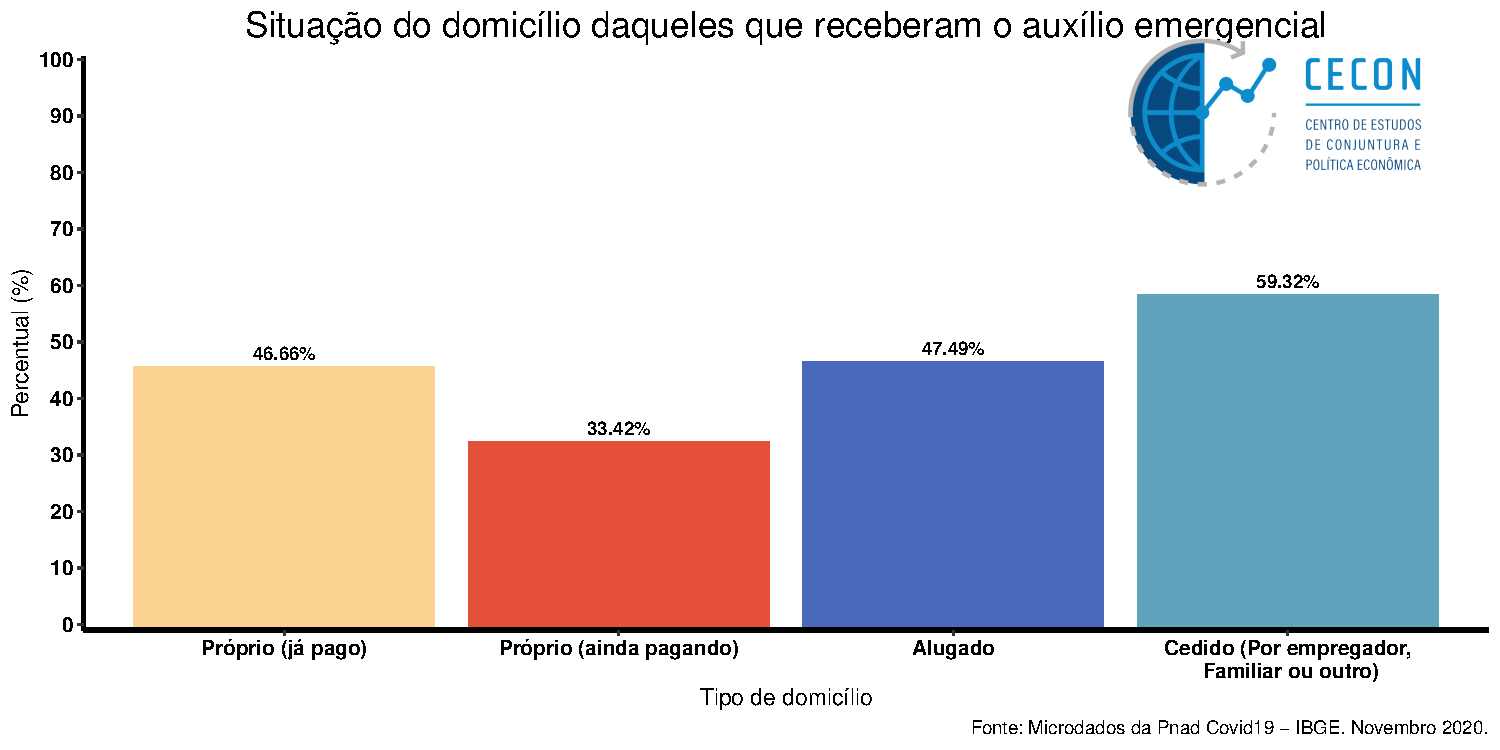
\includegraphics[width=.9\linewidth]{./figs/PNAD_COVID/auxilio_domicilio.pdf}
\end{center}
\subsection*{Auxilio - Sexo e Cor}
\label{sec:org85a489d}
\begin{center}
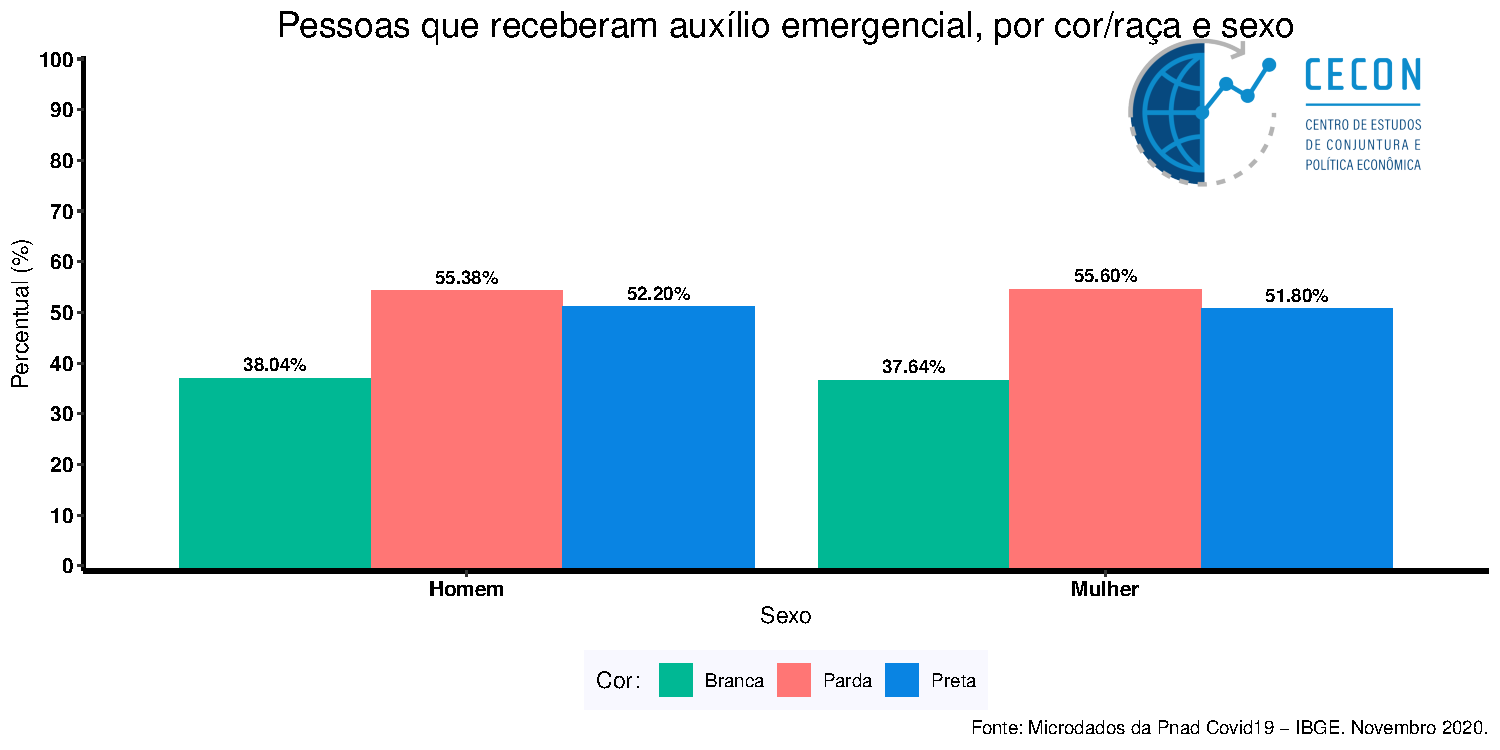
\includegraphics[width=.9\linewidth]{./figs/PNAD_COVID/auxilio_cor_sexo.pdf}
\end{center}


\section*{IMF Fiscal Monitor}
\label{sec:org13cae6b}
\subsection*{Medidas fiscais em \% do PIB}
\label{sec:org897f850}

\begin{center}
\includegraphics[width=.9\linewidth]{./figs/IMF/FiscalMonitor_Covid.pdf}
\end{center}

\subsection*{Medidas fiscais em \% do PIB: Setor de saúde/Outros setores}
\label{sec:orgbf7cb24}

\begin{center}
\includegraphics[width=.9\linewidth]{./figs/IMF/FiscalMonitor_Covid_ratio.pdf}
\end{center}

\subsection*{Medidas fiscais em \% do PIB: Setor de saúde/Total}
\label{sec:org9b4b182}

\begin{center}
\includegraphics[width=.9\linewidth]{./figs/IMF/FiscalMonitor_Covid_total.pdf}
\end{center}

\section*{World Economic outlook}
\label{sec:org591dacf}


\subsection*{GDP vs Lockdown}
\label{sec:org483b167}
\begin{table}[htbp]
\caption{\label{IMF_fig_1}GDP Forecast Errors in 2020:H1 and Lockdown Stringency}
\centering
\begin{tabular}{lll}
\hline
Países (ISO3) & 2020:H1 Erro da previsão do PIB (\%) & Rigidez do Lockdown (índice, média de 2020:H1)\\
\hline
AUS & -4,54 & 37,21\\
AUT & -9,11 & 37,13\\
BEL & -9,65 & 41,34\\
BRA & -8,71 & 44,01\\
CAN & -8,81 & 40,92\\
CHL & -5,71 & 41,76\\
CHN & -7,82 & 62,36\\
COL & -10,70 & 49,59\\
HRV & -9,36 & 40,25\\
CZE & -8,87 & 34,38\\
DNK & -6,03 & 39,22\\
EST & -6,54 & 31,58\\
FIN & -5,24 & 28,49\\
FRA & -13,44 & 48,72\\
DEU & -7,04 & 35,39\\
GRC & -10,79 & 39,91\\
HKG & -4,45 & 43,62\\
HUN & -8,91 & 38,69\\
IND & -15,70 & 51,69\\
IDN & -6,09 & 42,06\\
IRL & -3,48 & 45,59\\
ISR & -6,44 & 49,81\\
ITA & -11,99 & 51,65\\
JPN & -6,27 & 24,21\\
KOR & -3,02 & 39,64\\
LVA & -7,49 & 33,94\\
LTU & -3,51 & 40,30\\
MYS & -12,54 & 40,67\\
MEX & -11,10 & 41,61\\
NLD & -6,49 & 40,82\\
NOR & -6,10 & 32,55\\
PER & -20,54 & 55,43\\
PHL & -15,14 & 58,33\\
POL & -6,56 & 40,53\\
PRT & -10,87 & 43,79\\
ROU & -7,04 & 44,54\\
RUS & -4,29 & 48,61\\
SRB & -4,59 & 40,73\\
SGP & -7,63 & 43,65\\
SVK & -10,39 & 40,44\\
SVN & -11,35 & 34,24\\
ZAF & -9,66 & 47,21\\
ESP & -14,65 & 42,21\\
SWE & -4,28 & 21,08\\
CHE & -6,16 & 37,10\\
TWN & -1,37 & 13,73\\
THA & -9,13 & 39,43\\
TUR & -5,42 & 42,28\\
UKR & -8,08 & 47,94\\
GBR & -12,91 & 38,99\\
USA & -6,44 & 43,14\\
VNM & -4,35 & 47,91\\
\hline
\end{tabular}
\end{table}
\begin{center}
\includegraphics[width=.9\linewidth]{./figs/IMF/GDP_Lockdown.pdf}
\end{center}



\subsection*{Lockdown: Voluntary vs Stringency}
\label{sec:orga9fb135}

\begin{table}[htbp]
\caption{\label{Vol_String}Impact of Lockdowns and Voluntary Social Distancing on Mobility during the First 90 Days of Each Country’s Epidemic}
\centering
\begin{tabular}{lll}
Economias & Rigidez do Lockdown & Distanciamento Social Voluntário (DSV)\\
\hline
Todas & -7,85 & -6,53\\
Avançadas & -8,07 & -10,62\\
Emergentes & -8,78 & -6,26\\
Renda baixa & -5,8 & -2,83\\
\hline
\end{tabular}
\end{table}

\begin{center}
\includegraphics[width=.9\linewidth]{./figs/IMF/Vol_String.pdf}
\end{center}

\subsection*{Sequencing of lockdown measures}
\label{sec:orga9c6536}
\begin{table}[htbp]
\caption{\label{Lock_measure}Sequencing of lockdown measures}
\centering
\begin{tabular}{lrrr}
\hline
Lockdown measures & Middle & Low & High\\
\hline
Stay-at-home orders & 18 & 10 & 27\\
Public transport closures & 16 & 7,5 & 25\\
Internal movement restrictions & 16 & 7 & 27\\
Workplace closures & 13 & 6 & 22\\
Gathering restrictions & 10 & 2 & 20\\
Public event cancellations & 6 & 1 & 14,5\\
School closures & 4,5 & 1 & 13,5\\
International travel controls & 1 & 0 & 9\\
\hline
\end{tabular}
\end{table}

\begin{center}
\includegraphics[width=.9\linewidth]{./figs/IMF/Lock_measures.pdf}
\end{center}

\section*{OECD Weekly tracker}
\label{sec:org1ba5099}
\subsection*{Informações adicionais}
\label{sec:org335b303}

Conforme sugere o Anexo A (p. 40) de \textcite{woloszko_2020_Tracking}, a semana considerada se inicia aos domingos.
Compara-se com a mesma semana do ano anterior cujos dias da semana são os mais próximos da data de referência do ano corrente.
Exemplo dado pelo autor (p. 43):

\begin{quote}
The log difference for, say, 03-01-2020, is obtained by taking the difference between the \(svi_{03-01-2020}\) and the log of a weighted average of the closest known values before and after 03-01-2019, that is 31-12-2018 and 07-01-2019.
\end{quote}


\subsection*{Tracker e contrafactual}
\label{sec:org405d9d1}
\begin{center}
\includegraphics[width=.9\linewidth]{./figs/Granulares/OCDE_Semanal.pdf}
\end{center}

\subsection*{Tracker e contrafactual (subplots)}
\label{sec:orga853061}
\begin{center}
\includegraphics[width=.9\linewidth]{./figs/Granulares/OCDE_Subplots.pdf}
\end{center}

\subsection*{Contrafactual}
\label{sec:orge4d2f71}
\begin{center}
\includegraphics[width=.9\linewidth]{./figs/Granulares/OCDE_Contrafactual.pdf}
\end{center}

\section*{Auxílio emergencial}
\label{sec:orgb7d225c}

\npdecimalsign{,}
\npthousandsep{.}
\nprounddigits{0}
\begin{figure}[h]
    \resizebox{\textwidth}{!}{%
    \begin{tabular}{l|n{5}{2}|n{5}{2}|n{5}{2}|n{5}{2}|n{5}{2}|n{5}{2}|n{5}{2}|n{5}{2}|n{5}{2}|n{5}{2}|n{5}{2}}
\hline\hline
\multirow{2}{*}{(R\$ em milhões)} &
  \multicolumn{5}{c|}{Auxílio Emergencial} &
  \multicolumn{4}{c|}{Extensão do Auxílio Emergencial} &
  \multicolumn{1}{c|}{\multirow{2}{*}{2020}} &
  \multicolumn{1}{c}{\multirow{2}{*}{\% PIB 2020}} \\\cline{2-10}
 &
  \multicolumn{1}{c|}{abr/20} &
  \multicolumn{1}{c|}{mai/20} &
  \multicolumn{1}{c|}{jun/20} &
  \multicolumn{1}{c|}{jul/20} &
  \multicolumn{1}{c|}{ago/20} &
  \multicolumn{1}{c|}{set/20} &
  \multicolumn{1}{c|}{out/20} &
  \multicolumn{1}{c|}{nov/20} &
  \multicolumn{1}{c|}{dez/20} &
  \multicolumn{1}{c|}{} &
  \multicolumn{1}{c}{} \\\hline
AE Total &
  35781,054122 &
  41187,560652 &
  44699,80172948 &
  45919,51720376 &
  45060,964856 &
  24001,64923417 &
  20896,05343287 &
  18522,98326748 &
  18496,42121275 &
  294566,00571051 &
  4,0 \\
AE PBF &
  15176,3958 &
  15200,424 &
  15217,0812 &
  15141,69 &
  15196,3308 &
  4494,105196 &
  4380,11041 &
  4315,80209145 &
  4267,628712 &
  93389,56820945 &
  1,3 \\
AE CadÚnico não PBF &
  7018,7244 &
  6951,8544 &
  6619,3056 &
  6610,6482 &
  6368,0328 &
  2920,1895 &
  2863,8336 &
  2830,8507 &
  2801,0811 &
  44984,5203 &
  0,6 \\
AE Aplicativo &
  13585,7946 &
  19035,1344 &
  22859,7522 &
  24158,1816 &
  23456,7612 &
  16553,6688 &
  13623,9447 &
  11355,6693 &
  11411,8881 &
  156040,7949 &
  2,1 \\
AE Judicial &
  0,0954 &
  0,1039 &
  3,61874648 &
  8,95339076 &
  39,796012 &
  33,64166317 &
  28,12061787 &
  20,61704003 &
  15,77913475 &
  150,72590506 &
  0,0 \\
 &
   &
   &
   &
   &
   &
   &
   &
   &
   &
   &
   \\
PBF 2019 abril a dezembro &
  2632,27853599999 &
  2677,539162 &
  2627,861441 &
  2609,28159000001 &
  2608,191765 &
  2561,39384200001 &
  2564,19320299999 &
  2520,210959 &
  2525,74600700001 &
  23327 &
   \\
PBF 2019 para 2020 &
   &
   &
   &
   &
   &
   &
   &
   &
   &
  24381 &
   \\
 &
   &
   &
   &
   &
   &
   &
   &
   &
   &
   &
   \\
``AE efetivo'' (sem despesa de PBF) &
   &
   &
   &
   &
   &
   &
   &
   &
   &
  270185 &
  3,6 \\
 &
   &
   &
   &
   &
   &
   &
   &
   &
   &
   &
   \\
Valor 2021 &
   &
   &
   &
   &
   &
   &
   &
   &
   &
  44000 &
  0,6 \\
Equivalente a set/out. 2020 &
   &
   &
   &
   &
   &
   &
   &
   &
   &
  44898 &\\\hline\hline
\end{tabular}
} 
\end{figure}

\section*{Mobilidade e políticas implementadas}
\label{sec:orga4fec90}

\begin{center}
\includegraphics[width=.9\linewidth]{./figs/COVID/Mobilidade_Policy_selected_C6.pdf}
\end{center}




\section*{Mobilidade, medidas adotadas, casos acumulados por estados brasileiros}
\label{sec:org3774128}

\subsection*{Número de casos por estados}
\label{sec:org7947a03}

\begin{minted}[frame=lines,fontsize=\scriptsize,linenos]{r}

df <- read_csv(
  "./clean/COVID/Estados/Merged_wide.csv",
  guess_max = 3000
) %>%
  mutate(C6 = factor(C6),
         C6 = fct_relevel(C6, "Dados indisponíveis", "Sem restrição", "Recomendado ficar\nem casa", "Proibido sair\n(Salvo exceções)", "Proibido sair")) %>%
  mutate(Estado = factor(Estado)) %>%
  group_by(Sigla)

name = paste0('./figs/COVID/Estados/', figname, ".pdf")

df_inf <- df %>%
  group_by(Estado) %>%
  summarise(vline = date[Pico==1])

df %>% ggplot(aes(x=date)) +
  geom_line(aes(y=new_cases_100K), color="red") +
  geom_vline(
    data = df_inf,
    mapping = aes(xintercept = vline),
    color = "black"
  ) +
  labs(
    y = "Novos casos por\n100 mil habitantes",
    x = ""
  ) +
  theme(axis.text.x = element_text(angle = 90, vjust = 0.5, hjust=1)) +
  scale_x_date(date_breaks = "2 months", date_minor_breaks = "2 weeks", date_labels = "%b/%y") +
  guides(fill=guide_legend(title="Estados Brasileiros")) +
      theme(
        axis.text.y.left = element_text(size = 14),
        axis.text.x = element_text(size = 12),
        axis.title.y.left = element_text(size = 14),
        strip.text = element_text( size = 12, face = "bold" )
      ) +
  facet_wrap(~Estado) ->fig

 fig <- ggdraw(fig) +
   draw_image(logo_file, x = 0.95, y = 0.15, hjust = 1, vjust = 1, width = 0.15, height = 0.1)
ggsave(name, width = 40, height = 30, units = "cm")
print(name)
\end{minted}

\begin{center}
\includegraphics[width=.9\linewidth]{./figs/COVID/Estados/Casos.pdf}
\end{center}

\subsection*{Número de mortes por estados}
\label{sec:org0f77d61}

\begin{minted}[frame=lines,fontsize=\scriptsize,linenos]{r}

df <- read_csv(
  "./clean/COVID/Estados/Merged_wide.csv",
  guess_max = 3000
) %>%
  mutate(C6 = factor(C6),
         C6 = fct_relevel(C6, "Dados indisponíveis", "Sem restrição", "Recomendado ficar\nem casa", "Proibido sair\n(Salvo exceções)", "Proibido sair")) %>%
  mutate(Estado = factor(Estado)) %>%
  group_by(Sigla)

name = paste0('./figs/COVID/Estados/', figname, ".pdf")

df_inf <- df %>%
  group_by(Estado) %>%
  summarise(vline = date[Pico==1])

df %>% ggplot(aes(x=date)) +
  geom_line(aes(
    y=zoo::rollapply(new_deaths_100K, 14, mean, align='right',fill=NA)
    ), color="red") +
  ## geom_vline(
  ##   data = df_inf,
  ##   mapping = aes(xintercept = vline),
  ##   color = "black"
  ## ) +
  labs(
    y = "Novas mortes por 100 mil habitantes",
    x = ""
  ) +
  theme(axis.text.x = element_text(angle = 90, vjust = 0.5, hjust=1)) +
  scale_x_date(date_breaks = "2 months", date_minor_breaks = "2 weeks", date_labels = "%b/%y") +
  guides(fill=guide_legend(title="Estados Brasileiros")) +
      theme(
        axis.text.y.left = element_text(size = 14),
        axis.text.x = element_text(size = 12),
        axis.title.y.left = element_text(size = 14),
        strip.text = element_text( size = 12, face = "bold" )
      ) +
  facet_wrap(~Estado) ->fig

 fig <- ggdraw(fig) +
   draw_image(logo_file, x = 0.95, y = 0.15, hjust = 1, vjust = 1, width = 0.15, height = 0.1)
ggsave(name, width = 40, height = 30, units = "cm")
print(name)
\end{minted}

\begin{center}
\includegraphics[width=.9\linewidth]{./figs/COVID/Estados/Mortes.pdf}
\end{center}

\subsection*{Número de casos acumulados por estados}
\label{sec:org14872cd}

\begin{minted}[frame=lines,fontsize=\scriptsize,linenos]{r}

df <- read_csv(
  "./clean/COVID/Estados/Merged_wide.csv",
  guess_max = 3000
) %>%
  mutate(C6 = factor(C6),
         C6 = fct_relevel(C6, "Dados indisponíveis", "Sem restrição", "Recomendado ficar\nem casa", "Proibido sair\n(Salvo exceções)", "Proibido sair")) %>%
  mutate(Estado = factor(Estado)) %>%
  group_by(Sigla)

name = paste0('./figs/COVID/Estados/', figname, ".pdf")

df_inf <- df %>%
  group_by(Estado) %>%
  summarise(vline = date[Pico==1])

df %>% ggplot(aes(x=date)) +
  geom_line(aes(y=cum_cases_100K), color="red") +
  ## geom_vline(
  ##   data = df_inf,
  ##   mapping = aes(xintercept = vline),
  ##   color = "black"
  ## ) +
  labs(
    y = "Casos acumulados por\n100 mil habitantes",
    x = ""
  ) +
  theme(axis.text.x = element_text(angle = 90, vjust = 0.5, hjust=1)) +
  scale_x_date(date_breaks = "2 months", date_minor_breaks = "2 weeks", date_labels = "%b/%y") +
  guides(fill=guide_legend(title="Estados Brasileiros")) +
      theme(
        axis.text.y.left = element_text(size = 14),
        axis.text.x = element_text(size = 12),
        axis.title.y.left = element_text(size = 14),
        strip.text = element_text( size = 12, face = "bold" )
      ) +
  facet_wrap(~Estado) ->fig

 fig <- ggdraw(fig) +
   draw_image(logo_file, x = 0.95, y = 0.15, hjust = 1, vjust = 1, width = 0.15, height = 0.1)
ggsave(name, width = 40, height = 30, units = "cm")
print(name)
\end{minted}

\begin{center}
\includegraphics[width=.9\linewidth]{./figs/COVID/Estados/Casos_Cum.pdf}
\end{center}

\subsection*{Número de mortes acumuadas por estados}
\label{sec:orga131dd7}

\begin{minted}[frame=lines,fontsize=\scriptsize,linenos]{r}

df <- read_csv(
  "./clean/COVID/Estados/Merged_wide.csv",
  guess_max = 3000
) %>%
  mutate(C6 = factor(C6),
         C6 = fct_relevel(C6, "Dados indisponíveis", "Sem restrição", "Recomendado ficar\nem casa", "Proibido sair\n(Salvo exceções)", "Proibido sair")) %>%
  mutate(Estado = factor(Estado)) %>%
  group_by(Sigla)

name = paste0('./figs/COVID/Estados/', figname, ".pdf")

df_inf <- df %>%
  group_by(Estado) %>%
  summarise(vline = date[Pico==1])

df %>% ggplot(aes(x=date)) +
  geom_line(aes(y=cum_cases_100K), color="red") +
  ## geom_vline(
  ##   data = df_inf,
  ##   mapping = aes(xintercept = vline),
  ##   color = "black"
  ## ) +
  labs(
    y = "Mortes acumulados por 100 mil habitantes",
    x = ""
  ) +
  theme(axis.text.x = element_text(angle = 90, vjust = 0.5, hjust=1)) +
  scale_x_date(date_breaks = "2 months", date_minor_breaks = "2 weeks", date_labels = "%b/%y") +
  guides(fill=guide_legend(title="Estados Brasileiros")) +
      theme(
        axis.text.y.left = element_text(size = 14),
        axis.text.x = element_text(size = 12),
        axis.title.y.left = element_text(size = 14),
        strip.text = element_text( size = 12, face = "bold" )
      ) +
  facet_wrap(~Estado) ->fig

 fig <- ggdraw(fig) +
   draw_image(logo_file, x = 0.95, y = 0.15, hjust = 1, vjust = 1, width = 0.15, height = 0.1)
ggsave(name, width = 40, height = 30, units = "cm")
print(name)
\end{minted}

\begin{center}
\includegraphics[width=.9\linewidth]{./figs/COVID/Estados/Mortes_Cum.pdf}
\end{center}

\subsection*{Novos casos e mortes - Brasil}
\label{sec:org3c7e863}


\begin{center}
\includegraphics[width=.9\linewidth]{./figs/COVID/Estados/Brasil.pdf}
\end{center}

\subsection*{Gráficos de mobilidade e política por estados}
\label{sec:org6e39568}

\subsection*{Boxplots de taxa de crescimento e tipo de isolamento}
\label{sec:org7ba84af}

\begin{center}
\includegraphics[width=.9\linewidth]{./figs/COVID/Estados/Boxplot_Isolamento.pdf}
\end{center}

\subsection*{Gráficos de mobilidade e política por estados para indicar quando houve medida adotada}
\label{sec:orge5f4f7d}

\begin{center}
\includegraphics[width=.9\linewidth]{./figs/COVID/Estados/Quando_Policy_selected_C6.pdf}
\end{center}
\end{document}
